\documentclass[notoc,numbers]{tufte-handout}

%\geometry{showframe}% for debugging purposes -- displays the margins



\newcommand{\bra}[1]{\left(#1\right)}

\usepackage{clrscode3e}
\usepackage[activate={true,nocompatibility},final,tracking=true,kerning=true,spacing=true,factor=1100,stretch=10,shrink=10]{microtype}
\usepackage{tikz}
\usetikzlibrary{calc,positioning}
\usepackage{amsmath,amsthm, amssymb}
\usepackage{enumitem}
\usepackage{braket}
\newenvironment{rcases}
{\left.\begin{aligned}}
{\end{aligned}\right\rbrace}
\usepackage{mathrsfs}
\usepackage[boxed,linesnumbered]{algorithm2e}
\usetikzlibrary{shapes}
\usetikzlibrary{positioning}
% Set up the images/graphics package
\usepackage{graphicx}
\setkeys{Gin}{width=\linewidth,totalheight=\textheight,keepaspectratio}
\graphicspath{{.}}
\title{Lecture Notes for CS 726 - Spring 2022}
\author[Eeshaan Jain]{Eeshaan Jain}
\date{\today}  % if the \date{} command is left out, the current date will be used

% The following package makes prettier tables.  We're all about the bling!
\usepackage{booktabs}
% The units package provides nice, non-stacked fractions and better spacing
% for units.
\usepackage{units}

% The fancyvrb package lets us customize the formatting of verbatim
% environments.  We use a slightly smaller font.
\usepackage{fancyvrb}
\fvset{fontsize=\normalsize}
% Small sections of multiple columns
\usepackage{multicol}
\usepackage{cancel}
\usepackage{multirow,array}
\usepackage{xcolor}
\definecolor{DarkRed}{RGB}{139,0,0}
\usepackage{hyperref}
\hypersetup{colorlinks=true, linkbordercolor=DarkRed,linkcolor=DarkRed}
%--------Theorem Environments--------
%theoremstyle{plain} --- default
\newtheorem{thm}{Theorem}
\newtheorem{cor}[thm]{Corollary}
\newtheorem{prop}[thm]{Proposition}
\newtheorem{lem}[thm]{Lemma}
\newtheorem{conj}[thm]{Conjecture}
\newtheorem{quest}[thm]{Question}
\newtheorem{claim}{Claim}

\theoremstyle{definition}
\newtheorem{defn}[thm]{Definition}
\newtheorem{defns}[thm]{Definitions}
\newtheorem{con}[thm]{Construction}
\newtheorem{exmp}[thm]{Example}
\newtheorem{jk}[thm]{Joke}
\newtheorem{exmps}[thm]{Examples}
\newtheorem{notn}[thm]{Notation}
\newtheorem{notns}[thm]{Notations}
\newtheorem{addm}[thm]{Addendum}
\newtheorem{exer}[thm]{Exercise}

\theoremstyle{remark}
\newtheorem{rem}[thm]{Remark}
\newtheorem{ans}[thm]{Answer}
\newtheorem{rems}[thm]{Remarks}
\newtheorem{warn}[thm]{Warning}
\newtheorem{sch}[thm]{Scholium}

\newcommand{\ind}{\rotatebox[origin=c]{90}{$\models$}}
\newcommand{\nimplies}{\;\not\nobreak\!\!\!\!\implies}
\newcommand{\Mod}[1]{\ (\text{mod}\ #1)}
\newcommand{\R}{\mathbb{R}}
\newcommand{\N}{\mathbb{N}}
\newcommand{\Q}{\mathbb{Q}}
\newcommand{\F}{\mathbb{F}}
\newcommand{\Z}{\mathbb{Z}}
\newcommand{\Prob}{\text{Pr}}
\renewcommand{\P}{\mathbb{P}}
\DeclareMathOperator{\Span}{Span}
\DeclareMathOperator{\val}{val}
\DeclareMathOperator{\comp}{comp}
\DeclareMathOperator{\im}{Im}
\DeclareMathOperator{\reg}{Reg}
\DeclareMathOperator{\odd}{Odd}
\DeclareMathOperator{\dist}{dist}
\DeclareMathOperator{\sbd}{sbd}
\DeclareMathOperator{\capac}{cap}
\DeclareMathOperator*{\argmax}{arg\,max} % thin space, limits underneath in displays

% These commands are used to pretty-print LaTeX commands
\newcommand{\doccmd}[1]{\texttt{\textbackslash#1}}% command name -- adds backslash automatically
\newcommand{\docopt}[1]{\ensuremath{\langle}\textrm{\textit{#1}}\ensuremath{\rangle}}% optional command argument
\newcommand{\docarg}[1]{\textrm{\textit{#1}}}% (required) command argument
\newenvironment{docspec}{\begin{quote}\noindent}{\end{quote}}% command specification environment
\newcommand{\docenv}[1]{\textsf{#1}}% environment name
\newcommand{\docpkg}[1]{\texttt{#1}}% package name
\newcommand{\doccls}[1]{\texttt{#1}}% document class name
\newcommand{\docclsopt}[1]{\texttt{#1}}% document class option name
\renewcommand{\listalgorithmcfname}{List of Algorithms}
\begin{document}
	
	\maketitle
	\begin{abstract}
		These are my lecture notes taken during the Advanced Machine Learning (CS 726) course at IIT Bombay during the Spring 2021 session.	\end{abstract}
	\tableofcontents
	\vspace{5mm}
	\listofalgorithms
	\newpage
	\section{Probabilistic Modeling}
\subsection{Probability Theory}
\marginnote{In a single coin toss, we have \[\Omega = \{\text{H}, \text{T}\}\]}
We will briefly review probability in a rigorous sense. \\We define events considering we have a space of possible outcomes denoted by $\Omega$. $\mathcal S$ is a set of measurable events, to which we assign probabilities, and each event $\alpha \in \mathcal S$ is a subset of $\Omega$. \\
The event space necessarily satisfies three properties - 
\begin{enumerate}
	\item It contains the empty event $\emptyset$ and the trivial event $\Omega$.
	\item It is closed under union, i.e if $\alpha, \beta \in \mathcal S$, so is $\alpha \cup \beta$.
	\item It is closed under complementation, i.e if $\alpha \in \mathcal S$, so is $\Omega - \alpha$. 
\end{enumerate}
\begin{defn}[Probability distribution]\label{defn:prob}
A probability distribution $P$ over $(\Omega, \mathcal S)$ is a mapping of events in $\mathcal S$ to real values satisfying 
\marginnote{A direct consequence of the properties is: \[P(\emptyset) = 0\]\[P(\alpha \cup \beta) = P(\alpha) + P(\beta) - P(\alpha \cap \beta)\]}
\begin{itemize}[leftmargin=1cm]
	\item[$\diamond$] $P(\alpha) \geq 0$ for all $\alpha \in \mathcal S$
	\item[$\diamond$] $P(\Omega) = 1$
	\item[$\diamond$] If $\alpha, \beta \in \mathcal S$ and $\alpha \cap \beta = \emptyset$, then $P(\alpha \cup \beta) = P(\alpha) + P(\beta)$
\end{itemize}
\end{defn}
Conditional probability answers the question - after learning that event $\alpha$ is true, how does our belief about $\beta$ change? Formally, we define
\begin{equation}
	P(\beta|\alpha) = \dfrac{P(\alpha \cap \beta)}{P(\alpha)}
\end{equation}
It can be checked that this satisfies Definition \ref{defn:prob} and is a probability distribution. Noting that $P(\alpha \cap \beta) = P(\alpha) P(\beta|\alpha)$, we define the chain rule of conditional probabilities
\begin{equation}
P(\alpha_1 \cap \cdots\cap \alpha_k) = P(\alpha_1) P(\alpha_2|\alpha_1) \cdots P(\alpha_k|\alpha_1\cap\cdots\cap\alpha_{k-1})
\end{equation}
We further define the Bayes' rule
\begin{equation}\label{eqn:bayes}
P(\alpha|\beta) = \dfrac{P(\beta|\alpha)P(\alpha)}{P(\beta)}
\end{equation}
Here, $P(\alpha|\beta)$ is called the \textit{posterior}, $P(\beta|\alpha)$ is the \textit{likelihood}, $P(\alpha)$ is the \textit{prior} and $P(\beta)$ is the \textit{marginal probability} of the structure in context. We can generalize Equation \ref{eqn:bayes} as
\begin{equation}
P(\alpha|\beta \cap \gamma) = \dfrac{P(\beta|\alpha \cap \gamma)P(\alpha|\gamma)}{P(\beta|\gamma)}
\end{equation}
Now, we formally define the notion of random variables, which intuitively can be considered to be attribute reporters.
\begin{defn}[Random Variable]
	A random variable $X$ is a \textit{measurable} function $X:\Omega \to \mathcal S$. The probability that $X$ takes values in a set $s \in \mathcal S$ is written as
	\begin{equation}
		\text{Pr}(X \in s) = \text{Pr}(\{\omega \in \Omega|X(\omega) \in s\})
	\end{equation}
\end{defn}
The marginal distribution over a random variable $X$ is the distribution over events that can be described using $X$, and is denoted by $P(X)$. More generally, if we want to describe a distribution over a set of random variables $\mathcal X = \{x_1, \cdots, x_n\}$ called the \textit{joint distribution} denoted as $P(x_1, \cdots, x_n)$. The full assignment to the variables is denoted as $\xi \in \text{Val}(\mathcal X)$. The space corresponding to the joint assignment in $\mathcal X$ is called the \textit{canonical outcome space}. \\
Now, we glance at independencies, a core component of Probabilistic Graphical Models.
\begin{defn}[Independence]
An event $\alpha$ is independent of an event $\beta$ denoted by $P \models (\alpha\ind\beta)$, if $P(\alpha|\beta) = P(\alpha)$ or $P(\beta) = 0$.
\end{defn}
\begin{prop}
A distribution satisfies $(\alpha \ind \beta)$ if and only if 
\begin{equation}
P(\alpha\cap\beta) = P(\alpha)P(\beta)
\end{equation}
\end{prop}
\begin{proof}
Skipped (hint: Use the definition of conditional probability).
\end{proof}
\begin{defn}[Conditional Indpendence]
An event $\alpha$ is conditionally independent of event $\beta$ given $\gamma$ in $P$, denoted by $P \models (\alpha \ind\beta|\gamma)$ if $P(\alpha|\beta\cap\gamma) = P(\alpha|\gamma)$ or if $P(\beta\cap\gamma) = 0$.
\end{defn}
\begin{prop}
$P$ satisfies $(\alpha\ind\beta|\gamma)$ if and only if 
\begin{equation}
P(\alpha \cap\beta|\gamma) = P(\alpha|\gamma)P(\beta|\gamma)
\end{equation}
\end{prop}
\begin{defn}
Let $\mathbf{X, Y, Z}$ be sets of random variables. $\mathbf X$ is conditionally independent of $\mathbf Y$ given $\mathbf Z$ in a distribution $P$ if $P$ satisfies $(\mathbf X = \mathbf x \ind \mathbf Y = \mathbf y | \mathbf Z = \mathbf z)$ for all values of $\mathbf x \in \text{Val}(\mathbf X), \mathbf y \in \text{Val}(\mathbf Y)$ and $\mathbf z \in \text{Val}(\mathbf Z)$. We say that the variables in $\mathbf Z$ are \textit{observed}. If $\mathbf Z$ is empty, then we say that $\mathbf X$ and $\mathbf Y$ are marginally independent.
\end{defn}
\begin{prop}
The distribution $P$ satisfies $(\mathbf X \ind \mathbf Y|\mathbf Z)$ if and only if 
\begin{equation}
	P(\mathbf X,\mathbf Y|\mathbf Z) = P(\mathbf X|\mathbf Z)P(\mathbf Y|\mathbf Z)
\end{equation}
\end{prop}
The following properties hold for conditional independencies:
\begin{enumerate}
	\item \textit{Symmetry:} $(\mathbf X \ind \mathbf Y|\mathbf Z) \implies (\mathbf Y \ind \mathbf X|\mathbf Z)$
	\marginnote{Decomposition can also be stated as \[\mathbf{X\ind \{Y, Z\} \implies X\ind Y, X\ind Z}\]}
	\item \textit{Decomposition:} $(\mathbf X \ind \mathbf{Y, W}|\mathbf Z) \implies (\mathbf X \ind \mathbf Y|\mathbf{Z})$
	\marginnote{Weak Union can also be stated as \[\mathbf{X\ind \{Y, Z\} \implies X\ind Y|Z}\] But note that, if $\mathbf{X\ind Y}$ and $\mathbf{Z}\;\cancel\ind\;\{\mathbf{X,Y}\}$ then it is not necessary to have $\mathbf{X\ind Y|Z}$}
	\item \textit{Weak Union:} $(\mathbf X \ind \mathbf Y, \mathbf W|\mathbf Z) \implies (\mathbf X \ind \mathbf Y|\mathbf Z,  \mathbf W)$
	\item \textit{Contraction:} $(\mathbf X \ind \mathbf W|\mathbf Z, \mathbf Y)\; \& \;(\mathbf X \ind \mathbf Y|\mathbf Z) \implies (\mathbf X \ind \mathbf Y, \mathbf W|\mathbf Z)$
	\marginnote{Contraction can also be stated as \[\mathbf{X\ind Y|Z, X\ind Z \implies X\ind \{Y,Z\}}\]}
\end{enumerate}
If our distribution is positive (i.e, for all non-empty $\alpha \in \mathcal S, P(\alpha) > 0$), we have another property
\begin{itemize}[leftmargin=1cm]
	\item[$\diamond$] \textit{Intersection:}  $(\mathbf X \ind \mathbf Y|\mathbf Z, \mathbf W)\; \& \;(\mathbf X \ind \mathbf W|\mathbf Z, \mathbf Y) \implies (\mathbf X \ind \mathbf Y, \mathbf W|\mathbf Z)$
\end{itemize}
\begin{thm}\label{thm:factor}
Consider $\mathcal{X} = \mathbf{\{X, Y, Z\}}$. Then $P\models (\mathbf X \ind \mathbf Y | \mathbf Z)$ if and only if we can write 
\begin{equation}
P(\mathcal X) = \phi_1(\mathbf{X, Z})\phi_2(\mathbf{Y, Z})
\end{equation}
\end{thm}
\begin{proof}
Skipped.
\end{proof}
\subsection{Probabilistic Graphical Models}
Given a set of $n$ random variables $\mathcal{X} = \{x_1, x_2, \cdots x_n\}$ where $n$ is large, we want to build a joint probability distribution $P$ over this set. Explicitly representing the joint distribution is computationally expensive, since just having binary values variables requires the joint distribution to specify $2^n-1$ numbers, and for more practical variables, the count is too large. \\
\marginnote{An example of a query can be - \texttt{Estimate the fraction of people with a bachelor's degree}.}
We want to efficiently represent, estimate and answer inference queries on the distribution.
\subsection{Alternatives to explicit joint distributions}
$\triangleright$ Can we assume all columns are independent? \textbf{NO} - this is obviously a very bad assumption. \\
\noindent$\triangleright$ Can we use data to detect highly correlated column pairs, and estimate their pairwise frequencies? \textbf{MAYBE} - but there might\\\noindent be too many correlated pairs, and the method is ad hoc.\\
\marginnote{Note that we write that a set $X$ is conditionally independent of $Y$ given $Z$, i.e $X \ind Y|Z$ if \[ \Prob(X|Y,Z) = \Prob(X|Z)\]}
\noindent To solve the above two not so good ways, we explore conditional independencies. It may be possible that $\texttt{income } \cancel{\ind} \texttt{ age}$ but \\\noindent$\texttt{income } {\ind} \texttt{ age}|\texttt{experience}$. \\
Probabilistic graphical models use a graph-based representation as the basis for compactly
encoding a complex distribution over a high-dimensional space. \\
It is convenient to represent the independence assumption using a graph. The so called graphical model has nodes as the variables (continuous or discrete), and the edges represent direct interaction. If we consider directed edges, we talk about Bayesian Networks, and if we consider undirected edges, we talk about Markov Random Fields. \\
Essentially the graphical model is a combination of the graph and potentials.
\begin{defn}[Potentials]
Potentials $\psi_c(\mathbf x_c)$ are scores for assignment of values to subsets c of directly
interacting variables. We factorize the probability as a product of these potentials, i.e
\begin{equation}
	\text{Pr}(\mathbf x = x_1, \cdots, x_n) \propto \prod \psi_s(\mathbf x_s)
\end{equation}
\end{defn}


	\section{Bayesian Networks}
Bayesian Networks, also referred to as \textit{directed graphical models} are a family of probability distributions that has a compact parameterization representable using a directed graph. \\
It is known that
\begin{equation}
\Prob(x_1, x_2, \cdots, x_n) = \Prob(x_1)\Prob(x_2|x_1)\Prob(x_3|x_2,x_1)\cdots\Prob(x_n|x_{n-1}, \cdots, x_1)
\end{equation}
A compact Bayesian Network is a distribution in which each factor in the above equation depends on the \textit{parent} variables represented by Pa($x_i$) for variable $x_i$. Thus, we have
\begin{equation}
\Prob(x_i|x_{i-1}, x_{i-2}, \cdots ,x_1) = \Prob(x_i|\text{Pa}(x_i))
\end{equation}
and the corresponding potentials at each node in terms of its parents are
\begin{equation}
\psi_i(x_i, \text{Pa}(x_i)) = \Prob(x_i, \text{Pa}(x_i))
\end{equation}
Thus,
\begin{equation}\label{eqn:factorization}
	\Prob(x_1, x_2, \cdots, x_n) = \prod_{i=1}^n \Prob(x_i|\text{Pa}(x_i))
\end{equation}
\marginnote{\begin{exmp}\label{exmp:bn-ind}
\end{exmp}}
\begin{marginfigure}
	\centering
	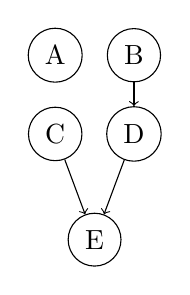
\begin{tikzpicture}[main/.style = {draw, circle}] 
		\node[main] (a) {A}; 
		\node[main] (b) [right of=a] {B};
		\node[main] (c) [below of=a] {C};
		\node[main] (d) [below of=b] {D};
		\node[main] (e) [below = of $(c)!0.5!(d)$] {E};
		\draw[->] (b) -- (d);
		\draw[->] (c) -- (e);
		\draw[->] (d) -- (e);
	\end{tikzpicture}
	\caption{Sample BN}
\end{marginfigure}
\marginnote{Consider the BN above. We will consider each variable at a time.
	\begin{itemize}
		\item[$\diamond$] $A$ has no parent, and has no descendent. Thus, \[ A \ind B, C, D, E\]
		\item[$\diamond$] $B$ has no parent, but has $D$ as a descendent. Thus, \[B \ind A, C\]
		\item[$\diamond$] $C$ has no parent, but has $E$ as a descendent. Thus, \[C \ind A, B, D\]
		\item[$\diamond$] $D$ has $B$ as a parent, and has $E$ as the descendent. Thus, \[D \ind A, C|B\]
		\item[$\diamond$] $E$ has $C$ and $D$ as parents, but has no descenent. Thus, \[I \ind A, B|C,D\]
	\end{itemize}
}
Consider the situation when each variable can take $d$ values. The naive approach gives us $\mathcal{O}(d^n)$ parameters. If we think of the potentials as probability tables (with the rows corresponding to Pa($x_i$)) and columns corresponding to the values of $x_i$, with entries as $\psi_{i}(x_i, \text{Pa}(x_i))$, we can notice that if $|\text{Pa}(x_i)| \leq k$, then the number of parameters are $\mathcal{O}(d^{k+1})$, and for $n$ variables, we have $\mathcal{O}(nd^{k+1})$, which provides us the compact representation.
\subsection{Definition}
Now we formally define these -
\begin{defn}[Bayesian Network]
A Bayesian Network is a directed graph $G = (V, E)$ together with 
\begin{itemize}[leftmargin=1cm]
	\item[$\diamond$] a random variable $x_i$ for each node $i \in V$
	\item[$\diamond$] a potential $\psi_i(x_i, \text{Pa}(x_i))$ for each node $i \in V$
\end{itemize}
\end{defn}
For a variable $x_i$ in our Bayesian Network $\mathcal G$, denote $\text{ND}(x_i)$ as the non-descendents of $x_i$. The following local conditional independencies hold in $\mathcal G$ - 
\begin{equation}
	x_i \ind \text{ND}(x_i) | \text{Pa}(x_i)
\end{equation}
Example \ref{exmp:bn-ind} shows the independencies in a simple Bayesian Network.
\begin{defn}[Factorization]	
Let $\mathcal{G}$ be a Bayesian Network graph over the variables $\{X_i\}_{i=1}^n$. We say that a distribution $P$ over the same space factorizes according to $\mathcal G$ if $P$ can be expressed as a product described in Equation \ref{eqn:factorization}. Such factorization is also known as the chain rule for Bayesian Networks, and is denoted as $\text{Factorize}(P, \mathcal G)$.
\end{defn}

\begin{defn}
Let $P$ be a distribution over $\mathcal X$. We define $\mathcal{I}(P)$ to be the set of independent assertions of the form $\mathbf X \ind \mathbf Y | \mathbf Z$ that hold in $P$.
\end{defn}
We can now write "$P$ satisfies the local independencies associated with $\mathcal  G$" as $\mathcal{I}_\ell(\mathcal G) \subseteq \mathcal{I}(P)$.
\begin{defn}[Independency-Map]
Let $\mathcal K$ be any graph object associated with a set of independencies $\mathcal{I}(\mathcal K)$. We call $\mathcal K$ an I-map for a set of independencies $\mathcal I$ if $\mathcal I(\mathcal K) \subseteq \mathcal I$.
\end{defn}
Thus for $\mathcal G$ to be an I-map for $P$, any independence that asserts in $\mathcal G$ must also assert in $P$, but $P$ can have additional independencies not reflected in $\mathcal G$.
\begin{rem}[Notation Alert]
Note that we will use the following interchangeably - $P$ satisfies the local conditional independencies satisfied by $\mathcal G$ and $\mathcal G$ is an I-map for $P$, i.e
\begin{equation}
	\text{Local-CI}(P, \mathcal G) \equiv \mathcal{I_\ell(G)} \subseteq \mathcal{I}(P)
\end{equation}
\end{rem}
\begin{thm}
Given a distribution $P(x_1, x_2, \cdots, x_n)$ and a directed acyclic graph (DAG) $\mathcal{G}$, 
\begin{equation}
\text{Local-CI}(P, \mathcal G) \Longleftrightarrow \text{Factorize}(P, \mathcal G)
\end{equation}
\end{thm}
\begin{proof}
($\implies$) We essentially need to show that if $\mathcal{G}$ is an I-map for $P$, then $P$ factorizes according to $\mathcal G$. Consider a topologically sorted order $x_1, x_2, \cdots, x_n$ in $\mathcal G$. $\text{Local-CI}(P, \mathcal G)$ tells us that $$\text{Pr}(x_i|x_{1}, \cdots, x_{i-1}) = \text{Pr}(x_i|\text{Pa}(x_i))$$
We can write
$$P(x_1, x_2, \cdots, x_n) = \prod_{i=1}^nP(x_i|x_1, \cdots, x_{i-1})$$
Each term in the product can be simplified due to the notion of Local-CI stated above, and we reach Equation \ref{eqn:factorization}, proving factorization. \\
($\impliedby$) Proof has been skipped.
\end{proof}
\subsection{Minimal Construction}
Our goal is to construct a minimal and correct BN $\mathcal G$ to represent $P$. A DAG $\mathcal G$ is correct if all Local-CIs that are implied in $\mathcal G$ hold in $P$, and a DAG $\mathcal G$ is minimal if we cannot remove any edge(s) from $\mathcal G$ and still\\ \noindent get a correct BN for $P$.
\\In the setting, we define our oracle $\mathscr{O}$ to whom we can ask any query of the type "\texttt{Is X $\ind$ Y|Z}?" pertaining to $P$ and get a boolean answer. We will query the oracle several times to build up our BN. The following algorithm constructs such a BN - \\
\begin{algorithm}[H]\label{alg:bn-con}
	\DontPrintSemicolon
	\textbf{Variables:} $x_1, x_2, \cdots, x_n \longleftarrow$ ordered variables in $\mathcal{X}$\;
	\textbf{Independencies:} $\mathcal I \longleftarrow$ set of independencies\;
	$\mathcal G \longleftarrow$ Empty graph over $\mathcal X$\;
	\For{$i=1$ to $n$}{
		$\mathbf U \longleftarrow \{x_1, \cdots, x_{i-1}\}$ \Comment{Set of candidate parents of $x_i$} \;
		\For{$U' \subseteq\{x_1, \cdots, x_{i-1}\}$}{
		\If{$U' \subset U$ and $(x_i \ind \{x_1, \cdots, x_{i-1}\} - U'|U')\in\mathcal I $}{
			$\mathbf{U} \longleftarrow U'$\;
			}	
	}
	\Comment{Now we have the minimal set $\mathbf{U}$ satisfying $(x_i \ind \{x_1, \cdots, x_{i-1}\} - \mathbf U|\mathbf U)$} \;
	\Comment{Now we set $\mathbf{U}$ to be the parents of $x_i$}\;
	\For{$x_j \in \mathbf U$}{
			Add $x_j \to x_i$ in $\mathcal G$
		}
	}
	\Return{$\mathcal{G}$}
	
	\caption{Minimal Bayesian Network Construction (I-Map)}
\end{algorithm}
We know sketch rough proofs for the claims of the algorithm.
\begin{thm}
The BN $\mathcal G$ constructed by algorithm \ref{alg:bn-con} is minimal, i.e we cannot remove any edge from the BN while maintaining the correctness of the BN for $P$.
\end{thm}
\begin{proof}
By construction. A subset of $\text{ND}(x_i)$ were available when we chose parents of $\mathbf U$ minimally.
\end{proof}
\begin{thm}
$\mathcal{G}$ constructed by the above algorithm is correct, i.e, the local-CIs induced by $\mathcal G$ hold in $P$.
\end{thm}
\begin{proof}
The construction is such that $\text{Factorize}(P, \mathcal G)$ holds everytime. Since $\text{Factorize}(P, \mathcal G) \implies \text{Local-CI}(P, \mathcal G)$, the constructed BN satisfies the local-CIs of $P$.
\end{proof}
\begin{quest}[Construction of BN]
Draw a Bayesian network over five variables $x_1,\cdots, x_5$ assuming the variable order $x_1, x_2, x_3, x_4, x_5$.
For this ordering, assume that the following set of local CIs hold in the distribution: 
\[x_1\ind x_2\quad x_3\ind x_2|x_1\quad x_4\ind x_1,x_3|x_2\quad x_5\ind x_1, x_2|x_3,x_4\]
\end{quest}
\begin{ans}
Due to the ordering, we begin by inserting $x_1$ into the BN. Then we follow Algorithm \ref{alg:bn-con} as follows:
\begin{enumerate}[leftmargin=1cm]
	\item $x_2$: Predecessor - $x_1$ \\
	\begin{itemize}[leftmargin=0.5cm]
	\item	\textit{Query 1} - Is $x_2 \ind x_1 | \emptyset$ ? :\textit{ Result 1} - True
	\end{itemize}
	Thus, $x_2$ has no parents.
	\item $x_3$: Predecessors - $x_1, x_2$
	\begin{itemize}[leftmargin=0.5cm]
		\item	\textit{Query 1} - Is $x_3 \ind \{x_1, x_2\} | \emptyset$ ? :\textit{ Result 1} - False
		\item	\textit{Query 2} - Is $x_3 \ind  x_2 | x_1$ ? :\textit{ Result 2} - True
	\end{itemize}
	Thus, $x_3$ has $x_1$ as a parent, and $x_2$ as a non-descendent.
	\item $x_4$: Predecessors - $x_1, x_2, x_3$
	\begin{itemize}[leftmargin=0.5cm]
		\item	\textit{Query 1} - Is $x_4 \ind \{x_1, x_2, x_3\} | \emptyset$ ? :\textit{ Result 1} - False
		\item	\textit{Query 2} - Is $x_4 \ind  \{x_2, x_3\} | x_1$ ? :\textit{ Result 2} - False
		\item	\textit{Query 3} - Is $x_4 \ind  \{x_1, x_3\} | x_2$ ? :\textit{ Result 3} - True
	\end{itemize}
	Thus, $x_4$ has $x_2$ as a parent, and $x_1, x_3$ as non-descendents.
	\begin{marginfigure}\label{fig:bn-example}
		\centering
		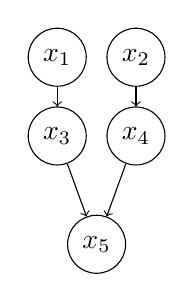
\begin{tikzpicture}[main/.style = {draw, circle}] 
			\node[main] (a) {$x_1$}; 
			\node[main] (b) [right of=a] {$x_2$};
			\node[main] (c) [below of=a] {$x_3$};
			\node[main] (d) [below of=b] {$x_4$};
			\node[main] (e) [below = of $(c)!0.5!(d)$] {$x_5$};
			\draw[->] (a) -- (c);
			\draw[->] (b) -- (d);
			\draw[->] (c) -- (e);
			\draw[->] (d) -- (e);
		\end{tikzpicture}
		\caption{BN Example}
	\end{marginfigure}
	\item $x_5$: Predecessors - $x_1, x_2, x_3, x_4$ \\
	Check that it has $x_3, x_4$ as parents and $x_1, x_2$ as non-descendents.
\end{enumerate}
Thus, finally we get the BN as in Figure \ref{fig:bn-example}
\end{ans}


\begin{rem}[Importance of ordering]
It is possible that a different ordering in $\mathcal X$ gives rise to a different BN, which although may be minimal, but may not be \textit{optimal}. A minimal BN is defined for a given ordering, while an optimal BN is defined over all orderings. Example \ref{exmp:bn-order} shows such a case.
\end{rem}
\begin{exmp}\label{exmp:bn-order}
To be added
\end{exmp}
\subsection{D-Separation}
Our goal is to know when we can guarantee $\mathbf X \ind \mathbf Y|\mathbf Z$ holds given a BN  $\mathcal G$. The further discussion provides some cases where we can guarantee $\mathbf X\; \cancel\ind\; \mathbf Y|\mathbf Z$.
\begin{marginfigure}
\begin{center}
	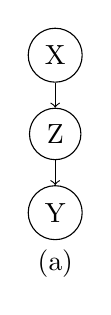
\begin{tikzpicture}[main/.style = {draw, circle}] 
	\node[main] (x) {X};
	\node[main] (z)[below of=x] {Z};
	\node[main] (y)[below of=z, label=below:(a)] {Y};
	\draw[->] (x) -- (z);
	\draw[->] (z) -- (y);
	\end{tikzpicture}
	\hspace{1cm}
	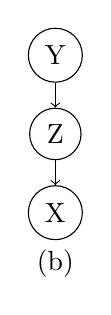
\begin{tikzpicture}[main/.style = {draw, circle}] 
		\node[main] (y) {Y};
		\node[main] (z)[below of=y] {Z};
		\node[main] (x)[below of=z, label=below:(b)] {X};
		\draw[->] (y) -- (z);
		\draw[->] (z) -- (x);
	\end{tikzpicture}
\end{center}
\caption{Causal and evidential effect}
\end{marginfigure}
\begin{marginfigure}
	\begin{center}
		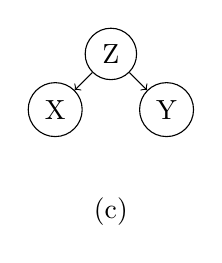
\begin{tikzpicture}[main/.style = {draw, circle}] 
			\node[main] (z) {Z};
			\node[main] (x)[below left of=z] {X};
			\node[main] (y)[below right of=z] {Y};
			\draw[->] (z) -- (x);
			\draw[->] (z) -- (y);
			\node (e) [below = of $(x)!0.5!(y)$] {(c)};
		\end{tikzpicture}
		\hspace{0.5cm}
		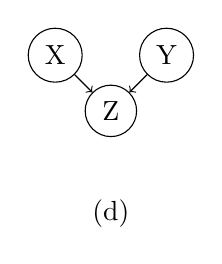
\begin{tikzpicture}[main/.style = {draw, circle}] 
			\node[main] (z) {Z};
			\node[main] (x) [above left of=z] {X};
			\node[main] (y)[above right of=z] {Y};
			\draw[->] (y) -- (z);
			\draw[->] (x) -- (z);
			\node (e) [below = of $(z)$] {(d)};
		\end{tikzpicture}
	\end{center}
	\caption{Common cause and common effect}
\end{marginfigure}
\begin{enumerate}
	\item \textbf{Direct Connection:} If there is an edge $X \to Y$, then regardless of any $\mathbf Z$, we can find examples where they influence each other.
	\item \textbf{Indirect Connection:} This means that there is a trail between the nodes in the graph. We consider the simple case when we a 3-node graph and $Z$ is between $X$ and $Y$. Consider the 4 diagrams to the left for reference.
	\begin{enumerate}
		\item \textit{Indirect causal effect:} $X$ cannot influence $Y$ via $Z$ if $Z$ is observed.
		\item \textit{Indirect evidential effect:} This is similar to the previous case as dependence is a symmetric notion. Thus, $X$ can influence $Y$ via $Z$, only if $Z$ is not observed.
		\item \textit{Common cause:} The conclusion is similar to (a) and (b).
		\item \textit{Common effect:} (v-structure) This case is a bit tricky to understand, but the crux is that $X$ can influence $Y$ when either $Z$ or one of $Z$'s descendents is observed.
	\end{enumerate}
If we have flow of influence from $X$ to $Y$ via $Z$, we say that the trail $X \rightleftharpoons Y \rightleftharpoons Z$ is active.
	\begin{equation}\label{eqn:dsep}
	\begin{split}
	&\begin{rcases}
		\text{Causal trail: }& X \to Z \to Y\\
		\text{Evidential trail: }&Y \to Z \to X \\
		\text{Common cause: }& X \leftarrow Z \to Y \\
	\end{rcases} \text{Active if and only if $Z$ is observed}\\
&\begin{rcases}
	\star \;\;	\text{Common effect: } X \to Z \leftarrow Y
\end{rcases} \\
&\hookrightarrow \text{Active if and only if $Z$ or one of $Z$'s descendent is observed}
	\end{split}
	\end{equation}
\end{enumerate}
Now, we can create a general notion of trails -
\begin{defn}
Let $\mathcal G$ be a BN, and $x_1 \rightleftharpoons \cdots \rightleftharpoons x_n$ be a trail in $\mathcal G$. Let $\mathbf Z \subset \{\text{observed variables}\}$. The trail is active given $\mathbf Z$ if
\begin{itemize}[leftmargin=1cm]
	\item[$\diamond$] Whenever we have a v-structure $x_{i-1} \to x_i \leftarrow x_{i+1}$, then $x_i$ or one of its descendents are in $\mathbf Z$
	\item[$\diamond$] No other node along the trail is in $\mathbf Z$.
\end{itemize}
We can see that if $x_1 \in \mathbf Z$ or $x_n \in \mathbf Z$, then the trail is inactive.
\end{defn}
\marginnote{Essentially in a DAG, $\mathbf Z$ d-separates $\mathbf X$ from $\mathbf Y$ if all paths $\mathcal P$ from any $\mathbf X$ to $\mathbf Y$ is blocked by $\mathbf Z$.\\A path $\mathfrak{P}$ is \textit{blocked} if it is inactive, i.e there is no flow of influence.}
\begin{defn}[d-separation]
Let $\mathbf X, \mathbf Y, \mathbf Z$ be three sets of nodes in $\mathcal G$. We say that $\mathbf X$ and $\mathbf Y$ are d-separated given $\mathbf Z$, i.e $\text{d-sep}_\mathcal{G}(\mathbf X; \mathbf Y|\mathbf Z)$ if there is no active trail between any node $x \in \mathbf X$ and $y \in \mathbf Y$ given $\mathbf Z$.
\end{defn}
\marginnote{We use the same notation as $\mathcal{I}(P)$ as we can show that the independencies in $\mathcal{I}(\mathcal G)$ are those guaranteed to hold for every distribution over $\mathcal G$ (Theorem \ref{thm:global-markov-ind}).}
\begin{defn}[Global Markov independencies]
The set 
\begin{equation}
\mathcal{I(G)} \overset{\mathrm{def}}{=} \{(\mathbf X \ind \mathbf Y | \mathbf Z): \text{d-sep}_\mathcal{G}(\mathbf X; \mathbf Y | \mathbf Z)\}
\end{equation}
denoting the set of independencies corresponding to d-separation is the set of global Markov independencies. 
\end{defn}
\begin{thm}\label{thm:global-markov-ind}
The d-separation test identifies the complete set of conditional independencies that hold in all distributions that conform to a given Bayesian Network.
\end{thm}
\begin{proof}
Skipped.
\end{proof}
Now, we look at another way to check d-separation over BNs, but first we define some terms.
\begin{defn}[Ancestral Graph]
Given a graph $G = (V,E)$ and a set of nodes to focus on, say $V^* \subseteq V$, the ancestral graph ${G}^A$ is a subgraph induced by $V^A = V^* \cup \mathcal{A}(V^*)$ where $\mathcal{A}(V^*)$ denotes the ancestors of $V^*$. Thus,
\begin{equation}
G^A = G\braket{V^A} = (V^A, \{(u,v) | (u, v) \in E \text{ and } u, v \in V^A\})
\end{equation}
\begin{defn}[Markov Blanket]
Given a random variable $Y$ in a random variable set $\mathcal X = {X_1, X_2, \cdots, X_n}$ , it's Markov Blanket is any subset $\mathcal S$ of $\mathcal X$, conditioned on which other variables are independent with $Y$, i.e
\begin{equation}
Y \ind \mathcal{X}\setminus\mathcal{S} | \mathcal S
\end{equation}
Thus, we can infer $Y$ from $\mathcal S$ itself, and the rest of the elements are redundant in observation.
\end{defn}
\marginnote{\begin{rem}\label{rem:bn-moral}Essentially we are finding an equivalent undirected graph for a DAG. We find all pairs of non-adjacent nodes having a common child, and add an undirected edge between them. Then we transform all directed edges in the resulting graph to undirected edges. \end{rem}}
\end{defn}
\begin{defn}[Moral graph]
A moral graph of a directed acyclic graph $G$ is an undirected graph in which each node of the original $G$ is now connected to its \textit{Markov Blanket}.
\end{defn}
\begin{algorithm}[H]\label{alg:bn-moral}
	\DontPrintSemicolon
	\textbf{Given:} Bayesian Network $\mathcal G$, Condition to check $\mathcal{C}$: $\mathbf X \ind \mathbf Y | \mathbf Z$ \;
	$\mathcal C \leftarrow$ False\;
	$G = (V,E) \leftarrow$ Underlying DAG in $\mathcal G$. \;
	$G^A = (V^A, E^A) \leftarrow$ Ancestral graph of $G$ \;
	$G^A_M = (V^A_M, E^A_M)\leftarrow$ Moral graph of $G^A$ using Note \ref{rem:bn-moral} \;
	\Comment{Delete the nodes in $\mathbf Z$ and all its connections}\;
	\For{$z \in \mathbf Z$}{
		$\Xi \leftarrow \{\}$\;
		\For{$u \in V$ such that $\xi=(u, z) \in E^A_M$}{
			$\Xi \leftarrow \Xi \cup \xi$\;
		}
		$E^A_M \leftarrow E^A_M \setminus \Xi$\;
		$V^A_M \leftarrow V^A_M \setminus \{z\}$\;
	}
	\If{$\mathbf X$ and $\mathbf Y$ are disconnected in the resulting graph}{
		$\mathcal C \leftarrow$ True\;
	}
	\caption{Checking for independence in a BN}
\end{algorithm}

	\section{Markov Random Fields}
\subsection{Intuition}
We saw previously that we cannot draw a \textit{perfect} I-map such that $\mathcal I(\mathcal G) = \mathcal{I}(P)$ for any distribution $P$ using directed graphical models. Such too is the case with undirected graphical models, but they help us to represent some of these independencies which directed graphs couldn't.\\
To be added.

\subsection{Cliques}
\begin{defn}[Complete Graph]
A complete graph is a simple undirected graph in which every pair of distinct vertices is connected by a unique edge.
\end{defn}

\begin{defn}[Clique]
A clique $C$ in an undirected graph $G = (V,E)$ is a subset of vertices, $C\subseteq V$ such that every two distinct vertices are adjacent. Thus, the subgraph induced by $C$, i.e $G\braket{C}$, is a complete graph.
\end{defn}

\begin{defn}[Maximal Clique]
A clique that cannot be extended by including one more adjacent vertex (i.e it does not exist exclusively within the vertex set of a larger clique) is a maximal clique.		
\end{defn}

\begin{defn}[Maximum Clique]
A maximum clique of a graph $G$, is a clique such that there is no other clique with more vertices.
\end{defn}
With each clique $C$, we associate a potential function $\psi$, which is a provisional function of its arguments that assigns a pre-probabilistic score of their joint distribution. It is to note that $\psi$ must be non-negative, but it shouldn't be interpreted as probability. 

\subsection{Gibbs Fields}
\begin{marginfigure}
\centering
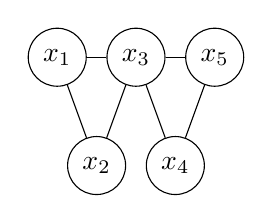
\begin{tikzpicture}[main/.style = {draw, circle}] 
	\node[main] (a) {$x_1$}; 
	\node[main] (c) [right of=a] {$x_3$}; 
	\node[main] (e) [right of=c] {$x_5$}; 
	\node[main] (b) [below = of $(a)!0.5!(c)$] {$x_2$};
	\node[main] (d) [below = of $(c)!0.5!(e)$] {$x_4$};
	\draw[-] (a) -- (c);
	\draw[-] (c) -- (e);
	\draw[-] (c) -- (b);
	\draw[-] (c) -- (d);
	\draw[-] (a) -- (b);
	\draw[-] (d) -- (e);
\end{tikzpicture}
\caption{A Gibbs Field}
\label{fig:gibbs-field-ex}
\end{marginfigure}
A Gibbs Field is a representation of a set of random variables and their relationships. An example is in Figure \ref{fig:gibbs-field-ex}. In this, the edges are undirected and imply some correlation between the connected nodes. \\
Consider clique potentials as $\psi_i(c_i)$. Then the joint probability for any set of random variables $\mathcal{X} = \{x_1, \cdots, x_n\}$ represented by a Gibbs Field can be written as a product of clique potentials
\begin{equation}
P(\mathcal X) = \dfrac{1}{Z} \prod_{c_i \in C} \psi_i(c_i)
\end{equation}
$Z$ is a normalizing constant required to create a valid probability distribution, i.e
\begin{equation}
Z = \sum_x \prod_{c_i \in C}\psi_i(C_i)
\end{equation}
\begin{rem}
For any Gibbs Field, there is a subset $\hat{C}$ of $C$ consisting of only maximal cliques, which are not proper subsets of any other cliques. We write the potentials for these maximal cliques as products of all potentials of their sub-cliques, and thus state the joint probability as
\begin{equation}
	P(\mathcal X) = \dfrac{1}{Z}\prod_{c_i \in \hat C} \hat{\psi}_i(c_i)
\end{equation}
\end{rem}
\subsection{Formal Definition}
\begin{defn}[Markov Random Field]
	A Markov Random Field (MRF) is a probability distribution $P$ over variables $x_1, \cdots, x_n$ defined by an undirected graph $G$ in which nodes correspond to variables $x_i$ and has the form
	\begin{equation}
		P(x_1, x_2, \cdots, x_n) = \dfrac{1}{Z}\prod_{c \in C} \psi_c(x_c)
	\end{equation}
	where 
	\begin{equation}
		Z = \sum_{x_1, \cdots, x_n}\prod_{c \in C} \psi_c (x_c)
	\end{equation}
	is the \textbf{\textit{partition function}} which is the normalizing constant ensuring the distribution sums to 1.
\end{defn}
\begin{marginfigure}
\centering
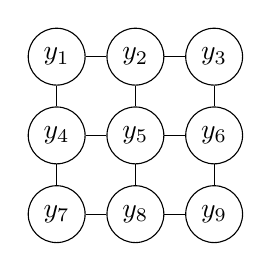
\begin{tikzpicture}[main/.style = {draw, circle}] 
	\node[main] (1) {$y_1$}; 
	\node[main] (2) [right of=1] {$y_2$}; 
	\node[main] (3) [right of=2] {$y_3$}; 
	\node[main] (4) [below of=1] {$y_4$}; 
	\node[main] (5) [right of=4] {$y_5$}; 
	\node[main] (6) [right of=5] {$y_6$}; 
	\node[main] (7) [below of=4] {$y_7$}; 
	\node[main] (8) [right of=7] {$y_8$}; 
	\node[main] (9) [right of=8] {$y_9$}; 
	\draw[-] (1) -- (2);
	\draw[-] (2) -- (3);
	\draw[-] (1) -- (4);
	\draw[-] (4) -- (5);
	\draw[-] (5) -- (6);
	\draw[-] (2) -- (5);
	\draw[-] (3) -- (6);
	\draw[-] (7) -- (8);
	\draw[-] (8) -- (9);
	\draw[-] (4) -- (7);
	\draw[-] (5) -- (8);
	\draw[-] (6) -- (9);
\end{tikzpicture}
\caption{Relations in image pixels}
\label{fig:markov-field-ex}	
\end{marginfigure}
As we saw earlier, if we have symmetric interactions, then UGMs become useful (such as labeling pixels in an image - see Figure \ref{fig:markov-field-ex}). Define $y_i = 1$ if the pixel is a part of the foreground, and 0 else. Taking cliques of size 1, we have the potential functions $\psi_1(0)$ to $\psi_9(0)$ and $\psi_1(1)$ to $\psi_9(1)$. Now considering cliques of size 2, we have $\psi(0,0), \psi(0, 1), \psi(1, 0)$ and $\psi(1,1)$. Thus we write
\begin{equation}
\text{Pr}(y_1, \cdots, y_9) \propto \prod_{k=1}^9 \psi_k(y_k) \prod_{(i,j) \in E(G)}\psi(y_i, y_j)
\end{equation}
\subsection{Conditional Independencies}
From now on, we will work on the UGM in Figure \ref{fig:markov-field-ex}. Let $$V = \{y_1, \cdots, y_9\}$$. We define three types of CIs in UGMs as follows
\begin{enumerate}
	\marginnote{In a graph $G$ with vertices $V = \{x_1, \cdots, x_n\}$, $\mathcal{N}(x_i)$ denotes the neighbors of $x_i$ in the graph}
	\item \textbf{Local CI:} $y_i \ind V - \mathcal{N}(y_i) - \{y_i\} | \mathcal{N}(y_i)$
	\[y_1 \ind y_3, y_5, y_6, y_7, y_8, y_9 | y_2, y_4\]
	\item \textbf{Pairwise CI:} $y_i \ind y_j | V - \{y_i, y_j\}$ if $(y_i, y_j) \notin E(G)$
	\[y_1 \ind y_3 | y_2, y_4, y_5, y_6, y_7, y_8, y_9\]
	\item \textbf{Global CI:} $\mathbf{X \ind Y | Z}$ if $\mathbf{Z}$ separates $\mathbf X$ and $\mathbf Y$ in the graph
	\[y_1, y_2, y_3 \ind y_7, y_8, y_9 | y_4, y_5, y_6\]
\end{enumerate}
Checking for CI in MRFs is much more easier than BNs. The way to check is through graph separability. Consider the example given in \textbf{Global CI}. If we remove $y_4, y_5$ and $y_6$ from the graph along with their edges, we see that the components $y_1, y_2, y_3$ is disconnected from $y_7, y_8, y_9$, and hence the CI holds.
\begin{thm}
Let $G$ be an undirected graph of $V = \{x_1, \cdots, x_n\}$ nodes, and let $P(x_1, \cdots, x_9)$ be a distribution. If $P$ is represented by $G$, that is, if it can be factorized as per the cliques of $G$, then $P$ will also satisfy the global-CIs of $G$. Thus
\begin{equation}
	\text{Factorize}(P, G) \implies \text{Global-CI}(P, G)
\end{equation}
\end{thm}
Note that for any arbitrary distribution, the converse doesn't hold, i.e in general for a distribution $P$
\begin{equation}
	\text{Factorize}(P, G) \nimplies \text{Global-CI}(P, G)
\end{equation}
\begin{marginfigure}
\centering
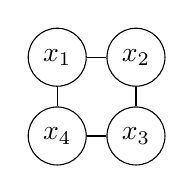
\begin{tikzpicture}[main/.style = {draw, circle}] 
	\node[main] (1) {$x_1$}; 
	\node[main] (2) [right of=1] {$x_2$}; 
	\node[main] (3) [below of=1] {$x_4$}; 
	\node[main] (4) [below of=2] {$x_3$}; 
	\draw[-] (1) -- (2);
	\draw[-] (4) -- (3);
	\draw[-] (1) -- (3);
	\draw[-] (2) -- (4);
\end{tikzpicture}
\caption{Sample UGM}
\label{fig:global-not-fact}		
\end{marginfigure}
We see this through a counter example. Consider the UGM in Figure \ref{fig:global-not-fact}, for the probability distribution $P(x_1, x_2, x_3, x_4)$ such that $P(x_1, x_2, x_3, x_4) = \frac{1}{8}$ when $x_1, x_2, x_3, x_4$ can take values from \\\noindent$\{0000, 1000, 1100, 1110, 1111, 0111, 0011, 0001\}$ else $0$. It can be manually checked that all 4 Global-CIs hold in the graph, for example $x_1 \ind x_3 | x_2, x_4$. Now consider the factors in the edges as $\psi(x_i, x_j)$. These will be positive, but that cannot represent the probability for $x_1, x_2, x_3, x_4 = 0101$. \\
Also, it is trivial to see that
\begin{equation}
	\text{Global-CI} \implies \text{Local-CI}
\end{equation}
But again through a counter example, we will show that the converse doesn't hold, i.e
\begin{equation}
	 \text{Local-CI} \nimplies \text{Global-CI}
\end{equation}
\begin{marginfigure}
	\centering
	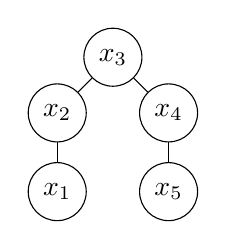
\begin{tikzpicture}[main/.style = {draw, circle}] 
		\node[main] (3) {$x_3$}; 
		\node[main] (4) [below right of=3] {$x_4$}; 
		\node[main] (2) [below left of=3] {$x_2$}; 
		\node[main] (5) [below of=4] {$x_5$}; 
		\node[main] (1) [below of=2] {$x_1$}; 
		\draw[-] (3) -- (2);
		\draw[-] (4) -- (3);
		\draw[-] (1) -- (2);
		\draw[-] (4) -- (5);
	\end{tikzpicture}
	\caption{Sample UGM}
	\label{fig:local-not-global}		
\end{marginfigure}
Consider a distribution over 5 binary variables $P(x_1, \cdots, x_5)$ where $x_1 = x_2, x_4 = x_5$ and $x_3 = x_2 \land x_4$. Consider $G$ as in Figure \ref{fig:local-not-global}. Notice that all 5 Local-CIs hold in the graph, for example $x_1 \ind \{x_3, x_4, x_5\} | x_2$. But notice that the graph also tells us that $x_2 \ind x_4 | x_3$, but this is not present in the distribution $P$. \\
We also notice that
\begin{equation}
	\text{Local-CI} \implies \text{Pairwise-CI}
\end{equation}
But again through a counter example, we show that the converse doesn't hold, i.e
\begin{equation}
 \text{Pairwise-CI}\nimplies 	\text{Local-CI}
\end{equation}
\begin{marginfigure}
	\centering
	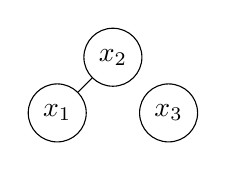
\begin{tikzpicture}[main/.style = {draw, circle}] 
		\node[main] (2) {$x_2$}; 
		\node[main] (1) [below left of=2] {$x_1$}; 
		\node[main] (3) [below right of=2] {$x_3$}; 
		\draw[-] (1) -- (2);
	\end{tikzpicture}
	\caption{Sample UGM}
	\label{fig:pairwise-not-local}		
\end{marginfigure}
Consider $P(x_1, x_2, x_3)$ defined over 3 binary variables such that $P(x_1,x_2,x_3) = \frac{1}{2}$ if $x_1=x_2=x_3$ and $0$ else. Let $G$ be as in Figure \ref{fig:pairwise-not-local}. See that both the Pairwise-CIs, i.e $x_1 \ind x_3 | x_2$ and $x_2 \ind x_3 | x_1$ hold in the graph, but the local CI $x_1 \ind x_3$ doesn't hold. \\
We have made a lot of statements about converses not holding in arbitrary distributions, but the natural question to arise is, can we find distributions where all the relations hold? The answer is yes, and is shown by the following theorem, also called the \textit{fundamental theorem of random fields} - 
\begin{thm}[Hammerseley Clifford Theorem]
If a positive distribution $P(x_1, \cdots x_n)$ confirms to the Pairwise-CIs of a UDGM $G$, then it can be factorized as per the cliques $C$ of $G$ as
\marginnote{A distribution $P(\mathbf x)$ is positive, if $P(\mathbf x) > 0 \; \forall \;\mathbf x$.}
\begin{equation}
	P(x_1, \cdots, x_n) \propto \prod_{C \in G} \psi_C(\mathbf{y}_C)
\end{equation}	
\end{thm}
\begin{proof}
Skipped.
\end{proof}
Thus, in summary, for any arbitrary distribution $P$ and UGM $H$,
\begin{equation}
	\begin{split}
	&\text{Factorize}(P, H) \implies \text{Global-CI}(P, H)\implies \\&\text{Local-CI}(P, H)\implies \text{Pairwise-CI}(P, H)
	\end{split}
\end{equation}
and if $P$ is positive, then
\begin{equation}
	\text{Pairwise-CI}(P, H) \implies \text{Factorize}(P, H)
\end{equation}
Hence, for a positive distribution, all three types of CIs are \textit{equivalent}.
\subsection{Minimal Construction}
The question to answer is, given a positive distribution $P(x_1, \cdots, x_n)$ as an oracle $\mathscr{O}$ to which we can ask the query - is $X\ind Y|Z$ and get a boolean answer, we need to draw a minimal and correct UGM $G$ to represent $P$. \\
Denote $V = \{x_1, x_2, \cdots, x_n\}$ as the set of all variables. We see that there are two methods to draw the UGM - 
\begin{enumerate}
	\item \textit{Using Pairwise-CIs:} For each pair of vertices $(x_i, x_j)$, if $x_i \ind x_j | V - \{x_i, x_j\}$ in $P$, add an edge between $x_i$ and $x_j$ in $G$.
	\item \textit{Using Local-CIs:} For each vector $x_i$, find the smallest subset $U$ such that $x_i \ind V - U - \{x_i\}|U$ in $P$. Then, add $U$ to $\mathcal{N}(x_i)$ in $P$.
\end{enumerate}
\begin{exmp}
	To be added.
\end{exmp}
We had seen Markov Blankets before, but we re-define them in terms of a UGM.
\begin{defn}[Markov Blanket]
The Markov Blanket (MB) of a variable $x_i$ is the smallest subset of variables $V$ that makes $x_i$ conditionally independent of others given the MB, i.e
\begin{equation}
x_i \ind V - MB(x_i) - \{x_i\} | MB(x_i)
\end{equation}
\end{defn}
\begin{thm}
The MB of a variable is always unique for a positive distribution.
\end{thm}
\begin{proof}
We will prove the following by contradiction. Let $x_i \in V$ and $M_1, M_2$ be two MBs. Let $\alpha = M_1 - M_2$ and $\beta = M_2 - M_1$, $M = M_1 \cap M_2$, $W = V - (M_1 \cup M_2)$. Note that, by definition, $x_i \ind V-M_2|M_2$ and $x_i \ind V-M_1|M_1$. Using this, we can write
\[x_i \ind W, \alpha|M, \beta \quad x_i \ind W, \beta|M,\alpha\]
For positive distributions, using intersection property, we can write
\[x_i \ind W, \alpha, \beta | M\]
This implies that $M$ is also a MB, but that is a contradiction since $M_1$ and $M_2$ were supposed to be minimal. Hence, the MB is unique.
\end{proof}
\marginnote{Interesetingly, UGMs were initially used to model interactions of atoms in gases and solids in 1800. A few other places where they are used are in 
\begin{enumerate}
	\item Markov Random Fields - Image Segmentation
	\item Conditional Random Fields - Information Extraction
	\item Social Networks
	\item Bio-informatics - Annotating active sites in proteins	 
\end{enumerate}
}
\begin{defn}[Immorality]
In a directed acyclic graph, the structure of the form $x \to y \leftarrow z$ is an immorality provided there is no edge between $x$ and $z$.
\end{defn}
With this, we can restate the equivalence of BNs - \\
\textit{Two BNs $\mathcal G_1$ and $\mathcal G_2$ are equivalent \textbf{iff} they have the same skeleton structure and the same set of immoralities}.
\subsection{Conversion to and from Bayesian Networks}
\begin{thm}
In a Bayesian Network $\mathcal G$, the Markov Blanket of a variable $x_i$ is given as
\begin{equation}
	MB(x_i) = \text{Pa}(x_i) \cup \text{Ch}(x_i) \cup \text{Sp}(x_i)
\end{equation}
where $\text{Pa}(x_i)$, $\text{Ch}(x_i)$ and $\text{Sp}(x_i)$ denote the parents, children and spouses (unmarried shared parent) of the children of $x_i$ (if exists).
\end{thm}
\begin{proof}
Only a flavor of the proof is provided. We have seen moralization of the Bayesian Network $\mathcal{G}$, and when we get $\mathcal{G}^M$ (i.e the moralized graph), notice that removing the parents, children and spouses disconnects the node from the graph.
\end{proof}
\begin{marginfigure}
	\centering
	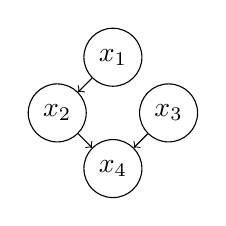
\begin{tikzpicture}[main/.style = {draw, circle}] 
		\node[main] (4) {$x_4$}; 
		\node[main] (2) [above left of=4] {$x_2$}; 
		\node[main] (3) [above right of=4] {$x_3$}; 
		\node[main] (1) [above right of=2] {$x_1$}; 
		\draw[->] (1) -- (2);
		\draw[->] (2) -- (4);
		\draw[->] (3) -- (4);
	\end{tikzpicture}
	\caption{Sample BN}
	\label{fig:bn-spouse-example}		
\end{marginfigure}
For example, in Figure \ref{fig:bn-spouse-example}, the MB of $x_2$ is given as
\[MB(x_2) = \{x_4\} \cup \{x_1\} \cup \{x_3\}\]
\begin{thm}
A Bayesian Network will have a perfect MRF if it has no immoralities.
\end{thm}
\begin{proof}
Skipped.
\end{proof}
We can ask the reverse question too. What condition should be posed on the MRF to have a perfect BN?
\begin{defn}[Chordal Graph]
A cordal graph is a simple graph in which every graph cycle of length four or greater has a cycle chord. 
\end{defn}
With this, we can state that
\begin{thm}
An MRF can be perfectly converted to a BN if and only if it is chordal.
\end{thm}
\begin{proof}
	Skipped.
\end{proof}
	\section{Inference Queries}
We have seen two major types of compact representations of joint probability distributions in terms of graphs. Summarizing the expressions of the joint distribution, we can write
\begin{align}
\text{For UGM: }\Prob(x_1, \cdots, x_n) &= \dfrac{1}{Z}\prod_C \psi_C(x_C) \\
\text{For DGM: }\Prob(x_1, \cdots, x_n) &= \prod_i \Prob(x_i|\text{Pa}(x_i))
\end{align}
We get a very compact representation if $\text{Pa}(x_i)$ is small. \\
Given a probability distribution $P$, we can ask two major types of queries - 
\begin{enumerate}
	\item \textit{Marginal probability queries over a sm`all subset of variables: }Given $P$, what is the marginal probability of $x_1$?.
	\begin{equation}
	\begin{split}
		\Prob(x_1) &= \sum_{x_2, \cdots, x_n} \Prob(x_1, \cdots, x_n) \\
		&= \sum_{x_2=1}^m \cdots \sum_{x_n=1}^m \Prob(x_1, \cdots, x_n)
	\end{split}
	\end{equation}
We can see that if each variable takes $m$ values, then the brute-force computation of the marginal probability will take $\mathcal{O}(m^{n-1})$ time.
\item \textit{Most likely labels of remaining variables (MAP queries): }Here, we ask questions of the form,
\begin{equation}
	\mathbf{x}^* = \argmax_{x_1, \cdots, x_n} \Prob(x_1, \cdots, x_n)
\end{equation}
An example of such a query could be - find the most likely entity labels of all words in a sentence.
\end{enumerate}
\begin{exmp}[Exact Inference]
Say we have a probability distribution over three binary variables as 
\[P(x_1, x_2, x_3) = \dfrac{1}{Z}\psi_{12}(x_1, x_2)\psi_{23}(x_2, x_3)\]
\begin{marginfigure}
	\centering
	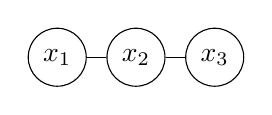
\begin{tikzpicture}[main/.style = {draw, circle}] 
		\node[main] (1) {$x_1$}; 
		\node[main] (2) [right of=1] {$x_2$}; 
		\node[main] (3) [right of=2] {$x_3$}; 
		\draw[-] (1) -- (2);
		\draw[-] (2) -- (3);
	\end{tikzpicture}
	\caption{UGM for $P(x_1, x_2, x_3)$}
	\label{fig:iq-p123-ugm}		
\end{marginfigure}
The UGM for this is shown in Figure \ref{fig:iq-p123-ugm}. Say we have the potential tables (each entry being $\psi_{ij}(a,b)$ representing the potential) as
\begin{center}
	\begin{tabular}{cc|c|c|}
		& \multicolumn{1}{c}{} & \multicolumn{2}{c}{$x_2$}\\
		& \multicolumn{1}{c}{} & \multicolumn{1}{c}{$0$}  & \multicolumn{1}{c}{$1$} \\\cline{3-4}
		\multirow{2}*{$x_1$}  & $0$ & $5$ & $2	$ \\\cline{3-4}
		& $1$ & $1$ & $4$ \\\cline{3-4}
	\end{tabular}
\qquad
\begin{tabular}{cc|c|c|}
	& \multicolumn{1}{c}{} & \multicolumn{2}{c}{$x_3$}\\
	& \multicolumn{1}{c}{} & \multicolumn{1}{c}{$0$}  & \multicolumn{1}{c}{$1$} \\\cline{3-4}
	\multirow{2}*{$x_2$}  & $0$ & $2$ & $10$ \\\cline{3-4}
	& $1$ & $5$ & $3$ \\\cline{3-4}
\end{tabular}
\end{center}
For example, we see that $\psi_{12}(0,0) = 5$. Let us find $P(x_1)$. 
\[P(x_1) =\dfrac{1}{Z} \sum_{x_2 \in \{0,1\}}\sum_{x_3 \in \{0,1\}}\psi_{12}(x_1, x_2)\psi_{23}(x_2, x_3)\]
We multiply the above two tables to get an intermediate potential distribution $\psi_{123}(x_1, x_2, x_3)$ and get a three dimensional table as follows (note that the columns denote $x_2$ and the rows denote $x_1$)
\begin{center}
	\begin{tabular}{cc|c|c|}
		& \multicolumn{1}{c}{} & \multicolumn{2}{c}{$x_3=0$}\\
		& \multicolumn{1}{c}{} & \multicolumn{1}{c}{$0$}  & \multicolumn{1}{c}{$1$} \\\cline{3-4}
		\multirow{2}*{}  & $0$ & $10$ & $10	$ \\\cline{3-4}
		& $1$ & $2$ & $20$ \\\cline{3-4}
	\end{tabular}
	\qquad
	\begin{tabular}{cc|c|c|}
		& \multicolumn{1}{c}{} & \multicolumn{2}{c}{$x_3=1$}\\
		& \multicolumn{1}{c}{} & \multicolumn{1}{c}{$0$}  & \multicolumn{1}{c}{$1$} \\\cline{3-4}
		\multirow{2}*{}  & $0$ & $50$ & $6$ \\\cline{3-4}
		& $1$ & $10$ & $12$ \\\cline{3-4}
	\end{tabular}
\end{center}
For example, $\psi_{12}(0,0)\psi_{23}(0,0) = 2\times5=10$. The next computation is to sum over $x_3$.
\[P(x_1) = \dfrac{1}{Z} \sum_{x_2 \in \{0,1\}} \psi_{12}^*(x_1, x_2)\]
The table after sum denoting $\psi_{12}^*(x_1, x_2)$ is
\begin{center}
	\begin{tabular}{cc|c|c|}
		& \multicolumn{1}{c}{} & \multicolumn{2}{c}{$x_2$}\\
		& \multicolumn{1}{c}{} & \multicolumn{1}{c}{$0$}  & \multicolumn{1}{c}{$1$} \\\cline{3-4}
		\multirow{2}*{$x_1$}  & $0$ & $60$ & $16$ \\\cline{3-4}
		& $1$ & $12$ & $32$ \\\cline{3-4}
	\end{tabular}
\end{center}
Now we eliminate $x_2$ by summing over the row values, thus finally
\[
\psi_1^*(x_1) = \dfrac{1}{Z}\begin{bmatrix}
	76 \\ 44
\end{bmatrix}
\]
Since this $P(x_1) = \psi_1^*(x_1)$, we immediately get to know that $Z = 76+44 = 120$. \\
Clearly, we see through the example that the calculation, even for three variables is cumbersome. Image doing this for thousands! \\
From the table in the above example, we can also calculate the assignment which gives the maximum probability. Note the $\psi_{123}$ table made, and see that $x_1=0, x_2=0, x_3=1$ has the score of $50$ giving the highest probability. But let us write this in a more algorithmic way
\[\mathbf{x^*} = \argmax_{x_2} \argmax_{x_2}\argmax_{x_3} \psi_{12}(x_1,x_2)\psi_{23}(x_2,x_3) \]
Let us construct the table $\psi_{12}^{\max} (x_1, x_2)$ from the $\psi_{123}$ table
\begin{center}
	\begin{tabular}{cc|c|c|}
		& \multicolumn{1}{c}{} & \multicolumn{2}{c}{$x_2$}\\
		& \multicolumn{1}{c}{} & \multicolumn{1}{c}{$0$}  & \multicolumn{1}{c}{$1$} \\\cline{3-4}
		\multirow{2}*{$x_1$}  & $0$ & $50$ for $x_3=1$ & $10$ for $x_3=0$ \\\cline{3-4}
		& $1$ & $10$ for $x_3=0$ & $20$ for $x_3=0$ \\\cline{3-4}
	\end{tabular}
\end{center}
Similarly, $\psi_1^{\max} (x_1)$ will be
\[
\begin{bmatrix}
	50 \text{ for $x_2=0, x_3=1$} \\ 20 \text{ for $x_2=1, x_3=0$} 
\end{bmatrix}
\]
At last, we can do an argmax over $x_1$ to get the assignment $x_1=0, x_2=0,x_3=1$ for the score of $50$.
\end{exmp}
Clearly, after the example, it is clear that we want to avoid the exponential overhead that brute-force approach applies.
\subsection{Exact Inference on Chains}
Consider the chain show in Figure \ref{fig:iq-chain}.
\begin{marginfigure}
	\centering
	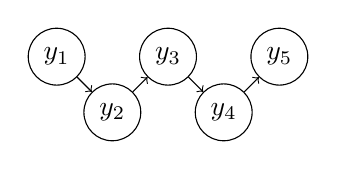
\begin{tikzpicture}[main/.style = {draw, circle}] 
		\node[main] (1) {$y_1$}; 
		\node[main] (2) [below right of=1] {$y_2$}; 
		\node[main] (3) [above right of=2] {$y_3$}; 
		\node[main] (4) [below right of=3] {$y_4$}; 
		\node[main] (5) [above right of=4] {$y_5$}; 
		\draw[->] (1) -- (2);
		\draw[->] (2) -- (3);
		\draw[->] (3) -- (4);
		\draw[->] (4) -- (5);
	\end{tikzpicture}
	\caption{Chain graph}
	\label{fig:iq-chain}		
\end{marginfigure}
We see that in the graph we would have potentials of the form $\psi_i(y_i, y_{i+1})$, and 
\begin{equation}
	\Prob(y_1, \cdots, y_n) = \prod_i \psi_i(y_i, y_{i+1})
\end{equation}
\textit{Note:} Since we don't have immoralities, the MRF is equivalent to the undirected version of the graph. Say we want to calculate 
\begin{equation}
\Prob(y_5=1) = \sum_{y_1, \cdots, y_4} \Prob(y_1, y_2, y_3, y_4, 1)
\end{equation}
The key idea to reducing computations is to push summations past the multiplications, i.e
\begin{equation}
\begin{split}
\Prob(y_5=1) &= \sum_{y_1, \cdots, y_4} \Prob(y_1, y_2, y_3, y_4, 1) \\
&= \sum_{y_1}\sum_{y_2}\sum_{y_3}\sum_{y_4} \psi_1(y_1, y_2)\psi_2(y_2,y_3)\psi_3(y_3,y_4)\psi_4(y_4,1) \\
&= \sum_{y_1}\sum_{y_2}\psi_1(y_1, y_2)\sum_{y_3}\psi_2(y_2, y_3)\sum_{y_4}\psi_3(y_3, y_4)\psi_4(y_4, 1) \\
&= \sum_{y_1}\sum_{y_2}\psi_1(y_1, y_2)\sum_{y_3}\psi_2(y_2, y_3)\mathcal{B}_3(y_3) \\
&= \sum_{y_1}\sum_{y_2}\psi_1(y_1, y_2) \mathcal{B}_2(y_2) \\
&= \sum_{y_1} \mathcal{B}_1(y_1) 
\end{split}
\end{equation}
We denote $\mathcal{B}_i(y_i)$ as the \textit{belief} which flows from node $i+1$ to $i$. This is an efficient computation. In general, if we have a chain with $n$ variables and each can take $m$ values, the above algorithm (breaking into beliefs) takes time in order of $\mathcal{O}(nm^2)$. \\
Notice that we did the efficient computation for chains, the natural question is, for what other graphs can this be done? \\
\begin{marginfigure}
	\centering
	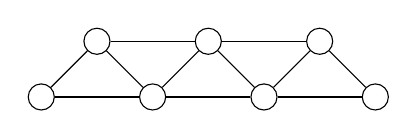
\begin{tikzpicture}[main/.style = {draw, circle}] 
		\node[main] (0) {};
		\node[main] (1) [above right of=0]{}; 
		\node[main] (2) [below right of=1] {}; 
		\node[main] (3) [above right of=2] {}; 
		\node[main] (4) [below right of=3] {}; 
		\node[main] (5) [above right of=4] {}; 
		\node[main] (6) [below right of=5] {}; 
		\draw[-] (0) -- (1);
		\draw[-] (1) -- (2);
		\draw[-] (0) -- (2);
		\draw[-] (1) -- (3);
		\draw[-] (2) -- (3);
		\draw[-] (2) -- (4);
		\draw[-] (3) -- (4);
		\draw[-] (3) -- (5);
		\draw[-] (4) -- (5);
		\draw[-] (4) -- (6);	
		\draw[-] (5) -- (6);
	\end{tikzpicture}
	\caption{Triangular graph}
	\label{fig:iq-triangle}		
\end{marginfigure}
Another one is shown in Figure \ref{fig:iq-triangle}. We define potential over each triangle (say $\psi_{123}$). If we follow a similar idea as the algorithm above, the time required for this computation will be $\mathcal{O}(nm^3)$.

\subsection{Hardness of Inference and 3-SAT}
The above discussion might lead to the thought that any graph $G$ which can be factorized into small clique sizes might have an efficient computation method (i.e polynomial time) of calculating the marginal probability.
\begin{marginfigure}
	\centering
	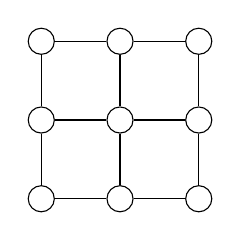
\begin{tikzpicture}[main/.style = {draw, circle}] 
		\node[main] (0) {};
		\node[main] (1) [right of=0]{}; 
		\node[main] (2) [right of=1] {}; 
		\node[main] (3) [below of=0] {}; 
		\node[main] (4) [below of=1] {}; 
		\node[main] (5) [below of=2] {}; 
		\node[main] (6) [below of=3] {}; 
		\node[main] (7) [below of=4] {}; 
		\node[main] (8) [below of=5] {}; 
		\draw[-] (0) -- (1);
		\draw[-] (1) -- (2);
		\draw[-] (0) -- (3);
		\draw[-] (1) -- (4);
		\draw[-] (2) -- (5);
		\draw[-] (3) -- (4);
		\draw[-] (5) -- (4);
		\draw[-] (3) -- (6);
		\draw[-] (4) -- (7);
		\draw[-] (5) -- (8);	
		\draw[-] (6) -- (7);
		\draw[-] (7) -- (8);
	\end{tikzpicture}
	\caption{Grid graph}
	\label{fig:iq-grid}		
\end{marginfigure}
 The answer sadly is no, and a counter example is the grid graph shown in Figure \ref{fig:iq-grid}. \\
 We will now reduce the $3$-SAT to inference in Bayesian Networks.
 \begin{defn}[$3$-SAT Problem]
 Given $n$ boolean variables $x_1, \cdots x_n$ such that $x_i \in \{T,F\}$. We define a literal $\ell$ to be the variable $x_i$ or its negation $\neg x_i$ or $\bar{x}_i$. Given a set of $K$ clauses $C_1, C_2, \cdots, C_K$ with each clause being
 \begin{equation} \label{eq:3-sat-clause}
 	C_j = \ell_{j_1} \lor \ell_{j_2} \lor \ell_{j_3}
 \end{equation}
The $3$-SAT problem is to decide if there exists an assignment of values to the $n$ variables such that 
\begin{equation}\label{eq:3-sat-sat}
	C_1 \land C_2 \land \cdots \land C_K = T
\end{equation}
 \end{defn}
\begin{exmp}\label{exmp:3-sat}
Consider $n=4, K=3$ and
\begin{align*}
	C_1 &= x_1 \lor \bar{x}_2 \lor \bar{x}_3 \\ 
	C_2 &= x_2 \lor x_3 \lor \bar{x}_4 \\
	C_3 &= x_4 \lor \bar{x}_1 \lor \bar{x}_2
\end{align*}
In this case, having all $x_i = T$ for $i = \{1, 2, 3, 4\}$ solves the problem.
\end{exmp}
In the above example, we by chance got lucky and solved the problem, but in general for a large number of variables, it is not possible to go over all possible combinations of values, since it requires an exponential amount of time. \\
Now we represent $3$-SAT as a Bayesian Network.
	\begin{marginfigure}
	\centering
	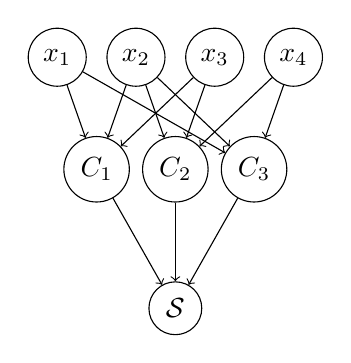
\begin{tikzpicture}[main/.style = {draw, circle}] 
		\node[main] (x1) {$x_1$}; 
		\node[main] (x2) [right of=x1] {$x_2$};
		\node[main] (x3) [right of=x2] {$x_3$};
		\node[main] (x4) [right of=x3] {$x_4$};
		\node[main] (c1) [below = of $(x1)!0.5!(x2)$] {$C_1$};
		\node[main] (c2) [below = of $(x2)!0.5!(x3)$] {$C_2$};
		\node[main] (c3) [below = of $(x3)!0.5!(x4)$] {$C_3$};
		\node[main] (s) [below = of c2] {$\mathcal S$};
     	\draw[->] (x1) -- (c1);
     	\draw[->] (x2) -- (c1);
     	\draw[->] (x3) -- (c1);
     	\draw[->] (x2) -- (c2);
     	\draw[->] (x3) -- (c2);
     	\draw[->] (x4) -- (c2);
     	\draw[->] (x4) -- (c3);
     	\draw[->] (x1) -- (c3);
     	\draw[->] (x2) -- (c3);
     	\draw[->] (c1) -- (s);
     	\draw[->] (c2) -- (s);
     	\draw[->] (c3) -- (s);
	\end{tikzpicture}
	\caption{3-SAT as BN}
	\label{fig:bn-3-sat}
\end{marginfigure}
Let us do that in a \textit{layer} sense. Let the first layer have all the variables as nodes and the next layer have all the clauses. Each clause will have 3 parents due to Equation \ref{eq:3-sat-clause}. Finally, the third layer would have $\mathcal S$, which is the satisfiability (Equation \ref{eq:3-sat-sat}), and it's parents would be all the clauses. Figure \ref{fig:bn-3-sat} shows the BN of Example \ref{exmp:3-sat}. \\
Coming back to the general setting, for each variable $x_i$, we denote
\begin{equation}
	\Prob(x_i) = \begin{cases}
		\frac{1}{2} & x_i=F \\
		\frac{1}{2} & x_i=T
	\end{cases}
\end{equation}

We also need to define $\Prob(C_j|\ell_{j_1}, \ell_{j_2}, \ell_{j_3})$. To do this, we assign a non-zero probability to only those which make $C_j=T$. This can be done uniformly (say out of the 8 assignments, 5 give a non-zero value, then $1$ for each of those assignments, and $0$ to rest - this is done because each $C_j$ is a deterministic function of the literals). Finally, we write the last probability $\Prob(\mathcal S|C_1, \cdots, C_K)$ as $1$ if $C_1, \cdots, C_K = T$, i.e all are true, and in the rest of the cases, we assign it as zero (note the difference here - the table for each $C_i$ had 8 rows, and the table for $\mathcal S$ has $2^K$ rows). The $2^K$ shows that it is not polynomial. This is again, not efficient. \\
One small change we can do is that instead of having a single $\mathcal S$ in the last layer, have $K-1$, such that each $\mathcal{S}_i$ is connected to $C_{i-1}$ and $C_i$ as parents, and each $\mathcal{S}_i$ is a parent of $\mathcal{S}_{i+1}$. This allows us to create the probability table as $\Prob(\mathcal{S}_j | \mathcal{S}_{j-1}, C_{j-1}, C_j)$ which represents the logic
\begin{equation}
	\mathcal{S}_j =  \mathcal{S}_{j-1} \land C_{j-1} \land C_j 
\end{equation} 
This allows each $\mathcal{S}_j$ with 8 variables, bringing in the needed efficiency. More specifically, the space required now is polynomial, since each $S_j$ requires only $2^4$ space, each $C_j$ requires $2^5$ space and each $x_j$ requires just constant (2) space. Thus overall the space required is $\mathcal{O}((K-1)\cdot2^4 + K\cdot 2^5+2)$
\\
Finally, if we can answer $\Prob(\mathcal{S}_j=1) > 0$ positively, then we know that a $3$-SAT assignment exists, else it does not.
\subsection{Variable Elimination on General Graphs}
We saw that using brute-force (i.e an exponential number of operations), we could calculate the normalizer $Z$. This is impractical, and hence we need a more efficient way to do so. Let's define the problem again - \\
Given an arbitrary set of potentials $\psi_C(x_C)$ in a graph $G$ where $C$ are the cliques in $G$, we need to find 
\[ Z = \sum_{x_1,\cdots,x_n} \prod_C \psi_C(x_C)\]
The algorithm to do so is as follows: \\
\begin{algorithm}[H]\label{alg:var-elim}
	\DontPrintSemicolon
	\textbf{Input:} Graph $G$\;
	\textbf{Variables:} $x_1, x_2, \cdots, x_n$ present in a \textit{good} ordering\;
	$\mathcal F \longleftarrow \{\psi_C(x_C)$ where $C=$ cliques in $G$\}  \;
	\For{$i=1$ to $n$}{
		$\mathcal F_i \longleftarrow$ factors in $\mathcal F$ containing $x_i$\;
		$\mathcal M_i \longleftarrow$ product of factors in $\mathcal F_i$\;
		$m_i \longleftarrow \sum_{x_i} \mathcal M_i$\;
		$\mathcal{F \longleftarrow (F}-\mathcal{F}_i) \cup \{m_i\}$\;
	}
	\caption{Variable Elimination}
\end{algorithm}
At the end, $\mathcal F$ consists of only a constant. Note that the product of factors isn't trivial, i.e we would need to multiply probability tables. To understand Algorithm \ref{alg:var-elim}, let's see an example.
\begin{exmp}\label{exmp:var-elim}
Say we have been given 5 variables, and the cliques are
\[\psi_{12}(x_1, x_2), \psi_{24}(x_2, x_4), \psi_{23}(x_2, x_3), \psi_{45}(x_4, x_5), \psi_{35}(x_3, x_5)\]
\begin{marginfigure}
	\centering
	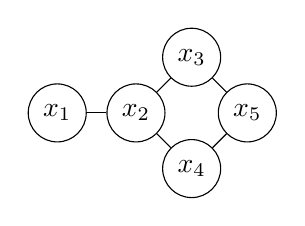
\begin{tikzpicture}[main/.style = {draw, circle}] 
		\node[main] (4) {$x_4$}; 
		\node[main] (2) [above left of=4] {$x_2$}; 
		\node[main] (5) [above right of=4] {$x_5$}; 
		\node[main] (3) [above right of=2] {$x_3$}; 
		\node[main] (1) [left of=2] {$x_1$}; 
		\draw[-] (1) -- (2);
		\draw[-] (2) -- (3);
		\draw[-] (2) -- (4);
		\draw[-] (4) -- (5);
		\draw[-] (3) -- (5);
	\end{tikzpicture}
	\caption{UGM for Example}
	\label{fig:iq-var-elim}		
\end{marginfigure}
The corresponding graph is in Figure \ref{fig:iq-var-elim}. We can see that 
\[Z = \sum_{x_1 \cdots x_5}\psi_{12}(x_1 x_2) \psi_{24}(x_2 x_4) \psi_{23}(x_2 x_3) \psi_{45}(x_4 x_5) \psi_{35}(x_3 x_5)\]
Say our good ordering is $x_1, x_2, x_3, x_4, x_5$. So we start
\begin{itemize}
	\item[$\diamond$] First variable $x_1$ - 
	\begin{align*}
	\mathcal{F}_1 &= \{\psi_{12}(x_1, x_2)\} \\
	\mathcal{M}_1(x_1, x_2) &= \psi_{12}(x_1, x_2) \\
	m_1(x_2) &= \sum_{x_1}\mathcal{M}_1 \\
	\mathcal{F} &= \{\psi_{24}(x_2, x_4), \psi_{23}(x_2, x_3), \psi_{45}(x_4, x_5), \psi_{35}(x_3, x_5), m_1(x_2)\}
	\end{align*}
\item[$\diamond$] Second variable $x_2$ - 
\begin{align*}
	\mathcal{F}_2 &= \{\psi_{24}(x_2, x_4), \psi_{23}(x_2, x_3), m_1(x_2)\} \\
	\mathcal{M}_2(x_2, x_3, x_4) &= \psi_{12}(x_2, x_4)\psi_{23}(x_2, x_3) m_1(x_2) \\
	m_2(x_3, x_4) &= \sum_{x_2}\mathcal{M}_2 \\
	\mathcal{F} &= \{\psi_{45}(x_4, x_5), \psi_{35}(x_3, x_5), m_2(x_3, x_4)\}
\end{align*}
\item[$\diamond$] Third variable $x_3$ - 
\begin{align*}
	\mathcal{F}_3 &= \{\psi_{35}(x_3, x_5), m_2(x_3, x_4)\} \\
	\mathcal{M}_3(x_3, x_4, x_5) &= \psi_{35}(x_3, x_5) m_2(x_3, x_4) \\
	m_3(x_4, x_5) &= \sum_{x_3}\mathcal{M}_3 \\
	\mathcal{F} &= \{\psi_{45}(x_4, x_5), m_3(x_4, x_5)\}
\end{align*}
\item[$\diamond$] Fourth variable $x_4$ - 
\begin{align*}
	\mathcal{F}_4 &= \{\psi_{45}(x_4, x_5), m_3(x_4, x_5)\} \\
	\mathcal{M}_4(x_4, x_5) &= \psi_{45}(x_4, x_5)m_3(x_4, x_5) \\
	m_4(x_5) &= \sum_{x_4}\mathcal{M}_4 \\
	\mathcal{F} &= \{m_4(x_5)\}
\end{align*}
\end{itemize}
\end{exmp}
The above example showed how $\mathcal F$ is a singleton set at the end. We can also modify Algorithm \ref{alg:var-elim} to get $\Prob(x_i)$ as follows - 
\begin{itemize}
	\item[$\diamond$] In line $1$ of Algorithm \ref{alg:var-elim}, we choose a good ordering such that $x_i$ is last
	\item[$\diamond$] The for loop in line 3 runs only for $n-1$ iterations
	\item[$\diamond$] After this, at the end, $\mathcal F$ will consist of unnormalized values, sum of which will give $Z$, and each term divided by $Z$ will give the required probability.
\end{itemize}
What if we want to compute the MAP query? For that, we do the follwing - 
\begin{itemize}
	\item[$\diamond$] In line 6, we have $\hat{m}_i = \max_{x_i} \mathcal{M}_i$ and we have to keep around the maximizing assignment
	\item[$\diamond$] In the end $\mathcal F$ consists of the required argmax.
\end{itemize}
\begin{thm}
The complexity of the Variable Elimination algorithm is $\mathcal{O}(nm^w)$ where $w$ is the maximum number of variables in any factor.
\end{thm}
\begin{proof}[Sketch of proof]
The bottleneck step in the algorithm's for loop is computing the product of factors, and in general if the factor has $\kappa$ variables, then the time to do the product will be $\mathcal{O}(m^\kappa)$.
\end{proof}
In Example \ref{exmp:var-elim}, we see that the time complexity is $\mathcal{O}(nm^3)$. If we started with $x_2$, our time complexity would've been $\mathcal{O}(nm^4)$.
\begin{marginfigure}
	\centering
	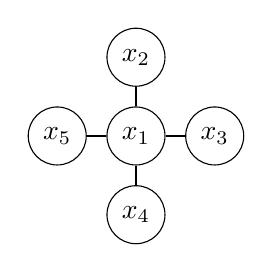
\begin{tikzpicture}[main/.style = {draw, circle}] 
		\node[main] (1)  {$x_1$}; 
		\node[main] (4) [below of=1]{$x_4$}; 
		\node[main] (2) [above of=1] {$x_2$}; 
		\node[main] (3) [ right of=1] {$x_3$}; 
		\node[main] (5) [ left of=1] {$x_5$}; 
		\draw[-] (1) -- (2);
		\draw[-] (1) -- (3);
		\draw[-] (1) -- (4);
		\draw[-] (1) -- (5);
		\draw[-] (1) -- (5);
	\end{tikzpicture}
	\caption{Star Graph}
	\label{fig:iq-star-graph}		
\end{marginfigure}
More interestingly, if we have a star graph (Figure \ref{fig:iq-star-graph}), and if we start with the centre node first, we encounter a very severe penalty in terms of time complexity. This elimination order will give you $\mathcal O(m^n)$ running time, while removing the non-central nodes first gives you just $\mathcal{O}(nm^2)$ running time.\\
Unfortunately, choosing the optimal elimination order is NP hard in general. But for chordal (triangulated) graphs, the algorithm is polynomial time. But another problem we stumble upon is that if our graph is not triangular, optimal triangulation is NP hard (but there exist many heuristics to do this in polynomial time).
\begin{defn}[Simplicial]
A vertex in a graph $G$ is simplicial if its neighbors form a complete set.
\end{defn}
\begin{thm}
Every triangulated graph is either complete or has at least two non-adjacent simplicial vertices.
\end{thm}
\begin{proof}
To be added.
\end{proof}
The goal is to find an optimal ordering for inferring $\Prob(x_1)$, which means $x_1$ should be last.\\
\begin{algorithm}[H]\label{alg:opt-order}
	\DontPrintSemicolon
	\textbf{Input:} Graph $G$, $n=$ number of vertices in $G$\;
	\For{$i=1$ to $n$}{
		$\pi_i \longleftarrow$ any simplicial vertiex in $G$ except $1$\;
		Remove $\pi_i$ from $G$\;
	}
	\Return{ordering $\pi_1, \cdots, \pi_{n-1}$}
	\caption{Optimal ordering for triangulated graph}
\end{algorithm}
\begin{marginfigure}
	\centering
	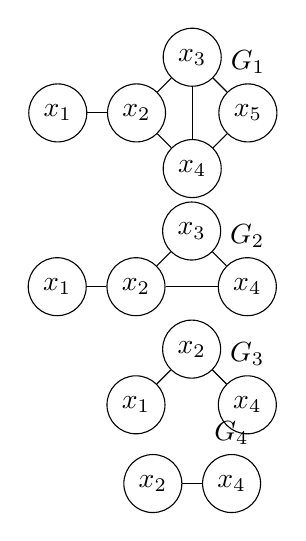
\begin{tikzpicture}[main/.style = {draw, circle}] 
		\begin{scope}
		\node[main] (4) {$x_4$}; 
		\node[main] (2) [above left of=4] {$x_2$}; 
		\node[main] (5) [above right of=4, label=$G_1$] {$x_5$}; 
		\node[main] (3) [above right of=2] {$x_3$}; 
		\node[main] (1) [left of=2] {$x_1$}; 
		\draw[-] (1) -- (2);
		\draw[-] (2) -- (3);
		\draw[-] (2) -- (4);
		\draw[-] (4) -- (5);
		\draw[-] (3) -- (5);
		\draw[-] (3) -- (4);
		\end{scope}
		\begin{scope}[yshift=-1.5cm, xshift=0.7cm]
		\node[main] (4) [label=$G_2$]{$x_4$}; 
		\node[main] (3) [above left of=4] {$x_3$}; 
		\node[main] (2) [below left of=3] {$x_2$}; 
		\node[main] (1) [left of=2] {$x_1$}; 
		\draw[-] (1) -- (2);
		\draw[-] (2) -- (3);
		\draw[-] (2) -- (4);
		\draw[-] (3) -- (4);
		\end{scope}
		\begin{scope}[yshift=-3cm, xshift=0.7cm]
			\node[main] (4) [label=$G_3$]{$x_4$}; 
			\node[main] (2) [above left of=4] {$x_2$}; 
			\node[main] (1) [below left of=2] {$x_1$}; 
			\draw[-] (1) -- (2);
			\draw[-] (2) -- (4);
		\end{scope}
	\begin{scope}[yshift=-4cm, xshift=-0.5cm]
		\node[main] (2){$x_2$}; 
		\node[main] (4) [label=$G_4$][right of=2] {$x_4$}; 
		\draw[-] (4) -- (2);
	\end{scope}
	\end{tikzpicture}
\caption{Sequence of graphs}
\label{fig:iq-opt-order}		
\end{marginfigure}
\begin{exmp}
Consider the triangulated graph $G_1$ given on the right for which we have to find the optimal ordering. We go over the iterations as follows
\begin{enumerate}
	\item  In $G_1$, we have $x_1$ and $x_5$ as simplicial vertices. Say we remove $x_5$ first, to get $G_2$.
	\item In $G_2$, we have $x_1, x_3$ and $x_4$ as the simplicial vertices. Say we remove $x_3$ to get $G_3$.
	\item In $G_3$, we have $x_1$ and $x_4$ as simplicial vertices. Say we remove $x_1$ to get $G_4$.
	\item In $G_4$ we have $x_2$ and $x_4$ as simplicial vertices.
	Say we remove $x_2$.
\end{enumerate}
The sequence of graphs is shown in Figure \ref{fig:iq-opt-order}. \\
Thus, finally we get the ordering $x_5, x_3, x_1, x_4, x_2$ as an optimal ordering. 
\end{exmp}
\subsection{Multiple Inference Queries}
The above subsection showed how we can calculate the optimal ordering and a single inference query. But say, we have been given a chain graph with potentials as $\psi_{i,i+1}(x_i, x_{i+1})$, say we need all $\Prob(x_1), \cdots, \Prob(x_n)$, can we do that faster? A no-brain method would be to use variable elimination $n$ times to get $\mathcal{O}(n^2m^2)$.
\begin{marginfigure}
	\centering
	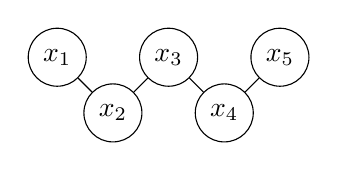
\begin{tikzpicture}[main/.style = {draw, circle}] 
		\node[main] (1) {$x_1$}; 
		\node[main] (2) [below right of=1] {$x_2$}; 
		\node[main] (3) [above right of=2] {$x_3$}; 
		\node[main] (4) [below right of=3] {$x_4$}; 
		\node[main] (5) [above right of=4] {$x_5$}; 
		\draw[-] (1) -- (2);
		\draw[-] (2) -- (3);
		\draw[-] (3) -- (4);
		\draw[-] (4) -- (5);
	\end{tikzpicture}
	\caption{Chain graph}
	\label{fig:iq-chain-graph}		
\end{marginfigure}
Say I have the chain graph in Figure \ref{fig:iq-chain-graph}. If we need to calculate $\Prob(x_1)$, we first remove $x_5$. This is followed by removing $x_4$, $x_3$ and $x_2$. \\
Now if we want to calculate $\Prob(x_2)$. We can reuse the computation done in removing $x_5, x_4$ and $x_3$. \\
We will see that if we skillfully reuse such computation, if each variable elimination run takes time $\mathfrak T$, the time for $n$ inference queries will take just $2\mathfrak T$.
\begin{rem}
Refer to Example \ref{exmp:var-elim}. In this notice that the arguments of $\mathcal M_i (\cdot)$ are cliques with \textit{induced} edges. For example, we have $\mathcal{M}_1(x_1, x_2)$ and clearly $\{x_1, x_2\}$ forms a clique. Second, we have $\mathcal{M}_2(x_2, x_3, x_4)$ and notice that when we add or \textit{induce} an edge between $x_2$ and $x_3$, $\{x_2, x_3, x_4\}$ forms a clique. This can be extended to all $\mathcal{M}_i(\cdot)$. For our notion of reusing, we are interested in the maximal cliques formed, and you can check that they refer to the cliques formed by the arguments of $\mathcal{M}_1, \mathcal{M}_2$ and $\mathcal{M}_3$.
\end{rem}
\subsection{Junction Trees}
The junction tree algorithm is an optimal general-purpose algorithm for \textbf{exact} marginal or MAP queries, and can simultaneously compute many such queries. It utilizes efficient data structures and overall has a complexity of $\mathcal O(m^wN)$ where $w$ is the size of the largest clique in the triangulated graph and each variable can take $m$ values. It is to note that 
\begin{itemize}
	\item[$\diamond$] Viterbi algorithm of Hidden Markov Models
	\item[$\diamond$] Forward-backward algorithm of Kalman Filters
\end{itemize}
are special cases of junction trees.
\begin{marginfigure}
	\centering
	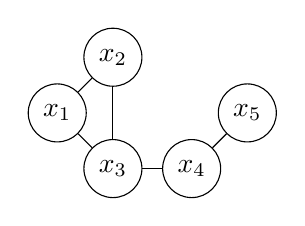
\begin{tikzpicture}[main/.style = {draw, circle}] 
		\node[main] (1)  {$x_1$}; 
		\node[main] (3) [below right of=1]{$x_3$}; 
		\node[main] (2) [above right of=1] {$x_2$}; 
		\node[main] (4) [right of=3] {$x_4$}; 
		\node[main] (5) [above right of=4] {$x_5$}; 
		\draw[-] (1) -- (2);
		\draw[-] (1) -- (3);
		\draw[-] (2) -- (3);
		\draw[-] (3) -- (4);
		\draw[-] (4) -- (5);
	\end{tikzpicture}
	\caption{Sample graph for JT}
	\label{fig:iq-jt-graph}		
\end{marginfigure}
\begin{defn}[Junction Tree]
Junction tree JT of a triangulated graph $G$ with nodes $x_1, \cdots, x_n$ is a tree where the nodes are the maximal cliques of $G$ and the edges obey the \textit{running intersection property}. This property states that if any two nodes contain variable $x_i$, then $x_i$ is present in every node in the unique path between them.
\end{defn}
\begin{marginfigure}
	\centering
	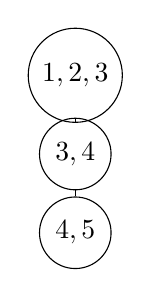
\begin{tikzpicture}[main/.style = {draw, circle}] 
		\node[main] (123)  {$1,2,3$}; 
		\node[main] (34) [below of=123]{$3,4$}; 
		\node[main] (45) [below of=34] {$4,5$}; 
		\draw[-] (123) -- (34);
		\draw[-] (34) -- (45);
	\end{tikzpicture}
	\caption{Junction Tree example}
	\label{fig:iq-jt-graph-jt}		
\end{marginfigure}
\begin{exmp}
For the graph given in Figure \ref{fig:iq-jt-graph}, we have the maximal cliques as $\{x_1, x_2, x_3\}, \{x_3, x_4\}, \{x_4, x_5\}$. Thus, the junction tree for the graph is given in Figure \ref{fig:iq-jt-graph-jt}
\end{exmp}
\begin{thm}
A graph will have a junction tree if and only if it is chordal.
\end{thm}
\begin{proof}
Skipped.
\end{proof}
\noindent\textbf{Construction of a junction tree}\\
If our graph is chordal, we have efficient polynomial time algorithms to create a JT. We first enumerate a set of maximal cliques covering our graph $G$, then we connect the cliques to get a tree satisfying the \textit{running intersection property}. Note that if our graph is non-triangulated, we need to triangulate it first using heuristics, since optimal triangulation is NP-hard.
\begin{defn}[Optimal triangulation]
A triangulation which gives rise to a JT where the size of the largest clique is smallest is called the optimal triangulation.
\end{defn}
\noindent A general method for finding heuristics is -
\begin{verbatim}
for i = 1 to n
	choose the vertex for which some score is minimum
	connect all neighbors of chosen vertex
	remove the chosen vertex from the graph
\end{verbatim}
Some heuristics of triangulation are
\begin{enumerate}
	\item Choose the vertex with smallest degree and connect all its neighbors
	\item Chose the vertex which will require the smallest number of edges to connect neighbors
\end{enumerate}
\begin{exmp}\label{exmp:jt-creation}
	Creation of a JT from a UGM:
	\begin{enumerate}
		\begin{marginfigure}
			\centering
			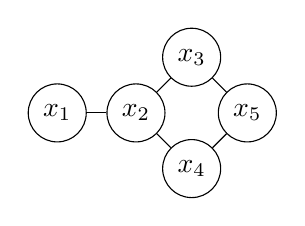
\begin{tikzpicture}[main/.style = {draw, circle}] 
				\node[main] (1)  {$x_1$}; 
				\node[main] (2) [right of=1] {$x_2$};
				\node[main] (3) [above right of=2]{$x_3$};  
				\node[main] (4) [below right of=2] {$x_4$}; 
				\node[main] (5) [above right of=4] {$x_5$}; 
				\draw[-] (1) -- (2);
				\draw[-] (2) -- (3);
				\draw[-] (2) -- (4);
				\draw[-] (3) -- (5);
				\draw[-] (4) -- (5);
			\end{tikzpicture}
			\caption{Non-chordal graph}
			\label{fig:iq-jt-exmp-unchordal}	
		\end{marginfigure}
	\begin{marginfigure}
		\centering
		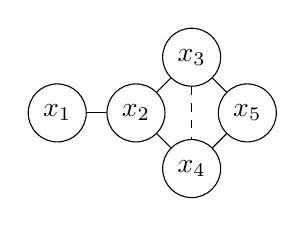
\begin{tikzpicture}[main/.style = {draw, circle}] 
			\node[main] (1)  {$x_1$}; 
			\node[main] (2) [right of=1] {$x_2$};
			\node[main] (3) [above right of=2]{$x_3$};  
			\node[main] (4) [below right of=2] {$x_4$}; 
			\node[main] (5) [above right of=4] {$x_5$}; 
			\draw[-] (1) -- (2);
			\draw[-] (2) -- (3);
			\draw[-] (2) -- (4);
			\draw[-] (3) -- (5);
			\draw[-] (4) -- (5);
			\draw[dashed] (3) -- (4);
		\end{tikzpicture}
		\caption{Chordal graph}
		\label{fig:iq-jt-exmp-chordal}	
	\end{marginfigure}
\begin{marginfigure}
	\centering
	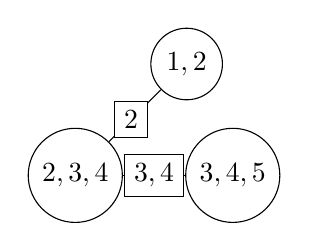
\begin{tikzpicture}[main/.style = {draw, circle}, sep/.style= {draw, rectangle}] 
		\node[main] (12)  {$1,2$}; 
		\node[sep] (2)  [below left of=12]{$2$}; 
		\node[main] (234) [below left of=2] {$2,3,4$};
		\node[sep] (34)  [right of=234]{$3,4$}; 
		\node[main] (345) [right of=34] {$3,4,5$};
		\draw[-] (12) -- (2);
		\draw[-] (2) -- (234);
		\draw[-] (234) -- (34);
		\draw[-] (34) -- (345);
	\end{tikzpicture}
	\caption{Clique-node graph}
	\label{fig:iq-jt-exmp-cliques}	
\end{marginfigure}
		\item Consider the graph in Figure \ref{fig:iq-jt-exmp-unchordal} as our starting graph. 
		
		\item We triangulate the graph to get the graph in Figure \ref{fig:iq-jt-exmp-chordal}. Notice that the maximal cliques are $C_1=\{x_1, x_2\}, C_2= \{x_2, x_3, x_4\}$ and $C_3=\{x_3, x_4, x_5\}$.
		
		\item These cliques act as nodes in our junction tree, and we connect the three cliques such that they satisfy the running intersection property. I have dropped the $x$ and just written the indices to avoid clutter. Note in Figure \ref{fig:iq-jt-exmp-cliques} that now we have two types of nodes - in circle we have the cliques, and in rectangles we have the \textit{separators}. Separators are variables present in the intersection of the nodes, thus
		\begin{equation}
		\text{Separator}(C_i, C_j) = C_i \cap C_j
		\end{equation}
	
		\item Now we assign potentials to all cliques. Note that from Example \ref{exmp:var-elim}, we had potentials $\psi_{12}, \psi_{23}, \psi_{24}, \psi_{35},\psi_{45}$. Thus here we can assign $\psi_{12}$ to $C_1$, $\psi_{23}, \psi_{24}$ to $C_2$ and $\psi_{35}, \psi_{45}$ to $C_3$. 
		\begin{rem}
		If we encounter any ambiguity in assigning potentials, i.e we can assign potentials to more than once clique-node, then we can arbitrarily assign it to any one.
		\end{rem}
	\end{enumerate}
\end{exmp}
\begin{thm}
Every triangulated graph has a simplicial vertex.
\end{thm}
\begin{proof}
Skipped.
\end{proof}
We now state the algorithm to find the maximal cliques in a triangulated graph \\
\begin{algorithm}[H]\label{alg:cliques-chordal}
	\DontPrintSemicolon
	\textbf{Input:} Triangulated graph $G$, $n=$ number of vertices in $G$\;
	\For{$i=1$ to $n$}{
		$\pi_i \longleftarrow$ any simplicial vertiex in $G$\;
		$C_i \longleftrightarrow \{\pi_i\} \cup \mathcal{N}(\pi_i)$\;
		Remove $\pi_i$ from $G$\;
	}
	\Return{the maximal cliques from $C_1, \cdots, C_n$}
	\caption{Finding maximal cliques in a chordal graph}
\end{algorithm}
\begin{thm}
A clique tree that satisfies the running intersection property maximized the number of separator variables.
\end{thm}
\begin{proof}
To be added.
\end{proof}
\begin{algorithm}[H]\label{alg:cliques-jt}
	\DontPrintSemicolon
	\textbf{Input:} Cliques $C_1, \cdots, C_k$\;
	Form a complete weighted graph $H$ with cliques as nodes and edge weights = size of the intersection of the two cliques it connects \;
	$T \longleftarrow$ maximum weight spanning tree of $H$\;
	\Return{$T$ as the junction tree}
	\caption{Forming a junction tree from a clique-node graph}
\end{algorithm}
Note that once we have the clique graph, we can make a weighted clique graph from that by adding $|\mathcal S|$ as the weight for each each between $C_i$ and $C_j$ where $\mathcal S = C_i \cap C_j$, and the problem of finding the junction tree boils down to finding the maximum weight spanning tree of the weighted graph.
\begin{exmp}
\begin{marginfigure}
	\centering
	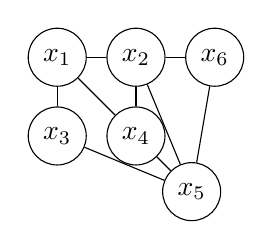
\begin{tikzpicture}[main/.style = {draw, circle}] 
		\node[main] (1)  {$x_1$}; 
		\node[main] (2) [right of=1] {$x_2$};
		\node[main] (3) [below of=1] {$x_3$};
		\node[main] (4) [below of=2] {$x_4$};
		\node[main] (5) [below right of=4] {$x_5$};
		\node[main] (6) [right of=2] {$x_6$};
		\draw[-] (1) -- (2);
		\draw[-] (1) -- (3);
		\draw[-] (1) -- (4);
		\draw[-] (2) -- (4);
		\draw[-] (2) -- (5);
		\draw[-] (2) -- (6);
		\draw[-] (3) -- (5);
		\draw[-] (4) -- (5);
		\draw[-] (5) -- (6);
	\end{tikzpicture}
	\caption{Undirected graph}
	\label{fig:iq-jt-exmp-ugm}	
\end{marginfigure}
Consider the undirected graph $H$ in Figure \ref{fig:iq-jt-exmp-ugm}. Say the potentials are defined over cliques of size 2. \\
To triangulate, say we pick a heuristic - smallest degree first. Start with $x_6$ and notice that its neighbors $x_2$ and $x_5$ are connected. Next we choose $x_3$ and connect $x_1$ and $x_5$. You can go on further, but notice that the graph is already triangulated (since on removing $x_1$ the graph becomes complete). Thus an ordering we can have is
\[x_6, x_3, x_1, x_2, x_5, x_4\]
Next we choose the maximal cliques. This can be done using Algorithm \ref{alg:cliques-chordal}. This gives the set of maximal cliques as
\begin{align*}
	C_1 &= \{x_3, x_1, x_5\}\\
	C_2 &= \{x_6, x_2, x_5\}\\
	C_3 &= \{x_1, x_2, x_4, x_5\}
\end{align*}
\begin{marginfigure}
	\centering
	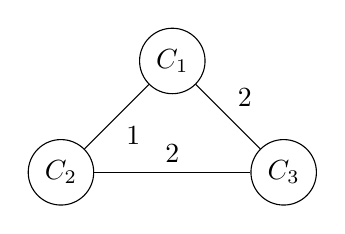
\begin{tikzpicture}[main/.style = {draw, circle}, node distance=2cm] 
		\node[main] (1)  {$C_1$}; 
		\node[main] (2) [below left of=1] {$C_2$};
		\node[main] (3) [below right of=1] {$C_3$};
		\draw[-] (1) to node[auto] {1} (2) ;
		\draw[-] (1) to node[auto] {2} (3) ;
		\draw[-] (2) to node[auto] {2} (3) ;
	\end{tikzpicture} 	
	\caption{Complete Weighted Graph}
	\label{fig:iq-jt-exmp-cwg}	
\end{marginfigure}
We then make the complete weighted graph as in Figure \ref{fig:iq-jt-exmp-cwg}. Clearly by removing the edge $C_1 - C_2$, we get the maximum spanning tree, and that gives the junction tree as shown in Figure \ref{fig:iq-jt-exmp-jt}.
\begin{marginfigure}
	\centering
	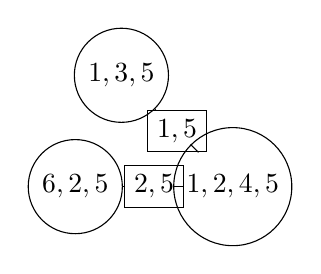
\begin{tikzpicture}[main/.style = {draw, circle}, sep/.style= {draw, rectangle}] 
		\node[main] (135)  {$1,3,5$}; 
		\node[sep] (5)  [below right of=135]{$1,5$}; 
		\node[main] (1245) [below right of=5] {$1, 2,4,5$};
		\node[sep] (25)  [left of=1245]{$2,5$}; 
		\node[main] (625) [left of=25] {$6, 2, 5$};
		\draw[-] (135) -- (5);
		\draw[-] (5) -- (1245);
		\draw[-] (625) -- (25);
		\draw[-] (25) -- (1245);
	\end{tikzpicture}
	\caption{Junction Tree}
	\label{fig:iq-jt-exmp-jt}	
\end{marginfigure}
To assign the potentials, we can assign $\psi_{13}, \psi_{35}$ to $C_1$, $\psi_{14}, \psi_{12}, \psi_{45}, \psi_{24}$ to $C_3$ and finally $\psi_{25}, \psi_{26}$ to $C_2$. The potential of a clique is the product of the potentials assigned to it.
\end{exmp}
\subsection{Message Passing}
Say each node $c$, which is a clique in the JT, sends a message $m_{c\to c'}(\cdot)$ to its neighbors $c'$ once it has messages from every other neighbor $\mathcal{N}(c) - \{c'\}$.
\begin{equation}
m_{c\to c'}(\mathbf{x}_s) = \sum_{\mathbf{x}_{c-s}}\psi_c(\mathbf x_c) \prod_{d \in \mathcal{N}(c) - \{c'\}} m_{d\to c} (\mathbf{x}_{d\cap c})
\end{equation}
For a MAP query, we can replace the $\sum$ with $\max$. Note that the $\sum$ sums over all the variables present in clique but not in separator. \\
We can write
\begin{equation}
	\Prob(\mathbf x_c) \propto \psi_c(\mathbf x_c) \prod_{d \in \mathcal{N}(c)} m_{d\to c}(\mathbf x_{d\cap c})
\end{equation}
And to get the marginal probability of any $x_i$, we can just sum over the rest, i.e
\begin{equation}
	\Prob(x_i) = \sum_{\mathbf x_c - x_i}\Prob(\mathbf x_c)
\end{equation}
\begin{exmp}
	\begin{marginfigure}
		\centering
		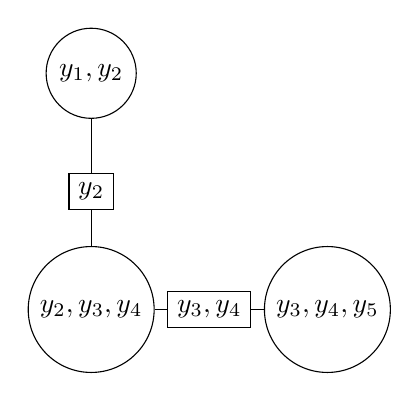
\begin{tikzpicture}[main/.style = {draw, circle}, sep/.style= {draw, rectangle}, node distance=1.5cm] 
			\node[main] (12)  {$y_1, y_2$};
			\node[sep] (2)  [below of=12]{$y_2$}; 
			\node[main] (234) [below of=2] {$y_2, y_3, y_4$};
			\node[sep] (34)  [right of=234]{$y_3,y_4$}; 
			\node[main] (345) [right of=34] {$y_3, y_4, y_5$};
			\draw[-] (12) -- (2);
			\draw[-] (2) -- (234);
			\draw[-] (234) -- (34);
			\draw[-] (34) -- (345);
		\end{tikzpicture}
		\caption{Junction Tree}
		\label{fig:iq-mp-exmp-jt}	
	\end{marginfigure}
Consider the JT shown in Figure \ref{fig:iq-mp-exmp-jt}. Note that we have edge potentials, and each clique has the product of such potentials present. Each node can send a message once it has messages from neighbors. \\
Initially, $C_1 = \{y_1, y_2\}$ or $C_3 = \{y_3, y_4, y_5\}$ can initiate the message passing since they have single neighbors. Thus, we have
\begin{enumerate}
	\item $C_1$ initiates message $m_{12\to234}(y_2) = \sum_{y_1} \psi_{12}(\mathbf y_{12})$ to $C_2 = \{y_2, y_3, y_4\}$.
	\item $C_3$ sends message $m_{345\to234}(\mathbf y_{34}) = \sum_{y_5}\psi_{345}(\mathbf y_{345})$ to $C_2$
	\item $C_2$ sends message $m_{234\to345} = \sum_{y_2} \psi_{234}(\mathbf y_{234})m_{12\to234}(y_2)$ to $C_3$
	\item $C_2$ sends message $m_{234\to12}(y_2) = \sum_{\mathbf{y_{34}}} \psi_{234}(\mathbf y_{234})m_{345\to234}(\mathbf y_{34})$ to $C_1$
\end{enumerate}
We also write that $\Prob(y_1) \propto \sum_{y_2} m_{234\to12}(y_2)$.
\end{exmp}
\begin{rem}[Intuition behind message passing]
Message from $c$ to $c'$ denotes the result of VE of potentials on the side of the tree that contains the clique $c$ but not $c'$ leaving only the separator variables $s = c\cap c'$.
\end{rem}
\subsection{Addition of Evidence}
In such queries, we have an evidence or conditioning set $\mathbf x_e$, and we need to find similar types of sub-queries shown before, i.e
\begin{enumerate}	\item $\Prob(x_1 | \mathbf{x}_e) = \sum_{x_2, \cdots, x_m} \Prob(x_1, \cdots, x_n| \mathbf{x}_e)$ \\
\item $\mathbf{x}^* | \mathbf{x}_e= \argmax_{x_1, \cdots, x_m} \Prob(x_1, \cdots, x_n | \mathbf{x}_e)$
\end{enumerate}
where $\{x_2, \cdots, x_m\} = V - \mathbf{x}_e - \{x_1\}$. The trick to add evidence is to change the potentials.
\begin{marginfigure}
	\centering
	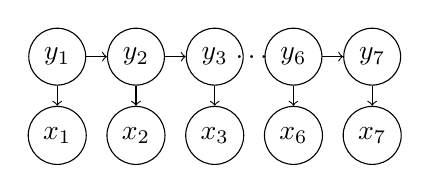
\begin{tikzpicture}[main/.style = {draw, circle}] 
		\node[main] (y1)  {$y_1$}; 
		\node[main] (y2) [right of=y1] {$y_2$};
		\node[main] (y3) [right of=y2] {$y_3$};
		\node[main] (y6) [right of=y3] {$y_6$};
		\node[main] (y7) [right of=y6] {$y_7$};
		\node[main] (x1) [below of=y1] {$x_1$};
		\node[main] (x2) [below of=y2] {$x_2$};
		\node[main] (x3) [below of=y3] {$x_3$};
		\node[main] (x6) [below of=y6] {$x_6$};
		\node[main] (x7) [below of=y7] {$x_7$};
		\node at ($(y3)!.5!(y6)$) {\ldots};
		\draw[->] (y1) -- (x1);
		\draw[->] (y1) -- (y2);
		\draw[->] (y2) -- (x2);
		\draw[->] (y2) -- (y3);
		\draw[->] (y3) -- (x3);
		\draw[->] (y6) -- (x6);
		\draw[->] (y6) -- (y7);
		\draw[->] (y7) -- (x7);
	\end{tikzpicture}
	\caption{Sample HMM}
	\label{fig:iq-xe-hmm}	
\end{marginfigure}
\begin{exmp}[Viterbi Algorithm]
Consider the Hidden Markov Model shown in Figure \ref{fig:iq-xe-hmm}. Define edge potentials as $\Prob(y_i|y_{i-1})$ and $\Prob(x_i|y_i)$. Also, let the evidence variables be $\mathbf{x} = x_1, \cdots, x_n = o_1, \cdots, o_n$. We need to find the most likely values of the hidden state variables $\mathbf y = y_1, \cdots, y_n$, i.e
\[\argmax_\mathbf{y} \Prob(\mathbf y | \mathbf x = \mathbf o)\]
We redefine the potentials as
\[\psi_i(y_{i-1}, y_i) = \Prob(y_i|y_{i-1})\Prob(x_i=o_i|y_i)\]
\begin{marginfigure}
	\centering
	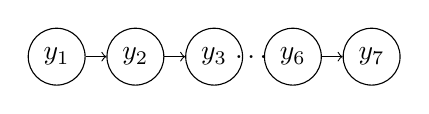
\begin{tikzpicture}[main/.style = {draw, circle}] 
		\node[main] (y1)  {$y_1$}; 
		\node[main] (y2) [right of=y1] {$y_2$};
		\node[main] (y3) [right of=y2] {$y_3$};
		\node[main] (y6) [right of=y3] {$y_6$};
		\node[main] (y7) [right of=y6] {$y_7$};
		\node at ($(y3)!.5!(y6)$) {\ldots};
		\draw[->] (y1) -- (y2);
		\draw[->] (y2) -- (y3);
		\draw[->] (y6) -- (y7);
	\end{tikzpicture}
	\caption{Sample HMM}
	\label{fig:iq-xe-rcg}	
\end{marginfigure}
Since we have fixed the observations of $x_i = o_i$, we have a 1D table instead of a 2D potential table. This gives the reduced chain graph as in Figure \ref{fig:iq-xe-rcg}. Now we use the message passing algorithm shown earlier, just replacing sum with max. For ease of calculation, only consider a three node chain, with the following probabilities:
\[\Prob(y_i = 0|y_{i-1}) = 
\begin{cases}
	0.9 &\text{if } y_{i-1} = 0 \\
	0.2 &\text{if } y_{i-1} = 1
\end{cases}
\]
\[\Prob(x_i = 0|y_{i}) = 
\begin{cases}
	0.7 &\text{if } y_{i} = 0 \\
	0.6 &\text{if } y_{i} = 1
\end{cases}
\]
Also, $\Prob(y_1 = 1) = 0.5$. Say our observations are
\[[x_1, x_2, x_3] = [0, 0, 0]\]
We want to calculate
\[\argmax \Prob(y_1, y_2, y_3 | x_1, x_2, x_3 = [0,0,0])\]
Now, we calculate the potential $$\psi_{12}(y_1, y_2)= \Prob(y_2|y_1)\Prob(x_1=0|y_1)\Prob(y_1)$$ 
\begin{center}
\begin{tabular}{cc|c|c|}
	& \multicolumn{1}{c}{} & \multicolumn{2}{c}{$\psi_{12}(y_1, y_2 ) $}\\
	& \multicolumn{1}{c}{} & \multicolumn{1}{c}{$0$}  & \multicolumn{1}{c}{$1$} \\\cline{3-4}
	\multirow{2}*{}  & $0$ & $0.9 \times 0.7 \times 0.5$ & $	0.1 \times 0.7 \times 0.5$ \\\cline{3-4}
	& $1$ & $0.2 \times 0.6 \times 0.5$ & $0.8\times 0.6 \times 0.5$ \\\cline{3-4}
\end{tabular}
\end{center}
Note that when we calculate $$\psi_{23}(y_2, y_3) = \Prob(y_3|y_2)\Prob(x_2=0|y_2)\Prob(x_3=0|y_3)$$
\end{exmp}
\begin{rem}[Approximate Inference]
Note the followings points:
\begin{itemize}
	\item[$\diamond$] Exact inference is NP hard. First define the tree width $w$ of a triangulated graph as one less than the size of the maximal clique. The complexity of exact inference is $\mathcal{O}(m^w)$.
	\item[$\diamond$] It is seen that real-life graphs produce large cliques on triangulation. For example, an $n\times n$ grid has a tree width of $n$. A Kalman filter on $K$ parallel state variables influencing a common observation variable has a tree width of size $K+1$.
\end{itemize}
\end{rem}
\subsection{Generalized Belief Propogation}
Here, we tr to run some kind of message passing algorithms on graphs which look like junction trees. Instead of creating an exact JT which satisfies the running intersection property, we try to create a cluster graph with two relaxations - 
\begin{enumerate}
	\item The nodes are arbitrary clusters instead of cliques in the chordal graph. We only ensure that all potentials are subsumed.
	\item Instead of adding separator nodes, we add a subset of intersecting variables so as to satisfy the running intersection property.
\end{enumerate}
\begin{exmp}
Consider the JT creation in Example \ref{exmp:jt-creation}. For that graph, we see that we get maximal clique size of 3. Suppose we want to maintain a clique size of 2. 
\begin{marginfigure}
	\centering
	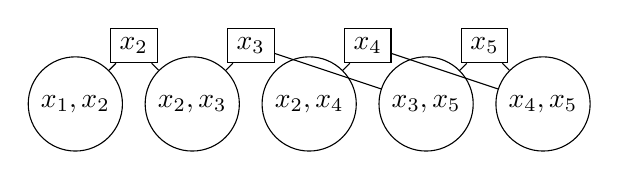
\begin{tikzpicture}[main/.style = {draw, circle}, sep/.style={draw, rectangle}, node distance=1.05cm] 
		\node[main] (12)  {$x_1, x_2$}; 
		\node[sep] (2) [above right of=12] {$x_2$};
		\node[main] (23) [below right of=2] {$x_2, x_3$}; 
		\node[sep] (3) [above right of=23] {$x_3$};
		\node[main] (24) [below right of=3] {$x_2, x_4$}; 
		\node[sep] (4) [above right of=24] {$x_4$};
		\node[main] (35) [below right of=4] {$x_3, x_5$}; 
		\node[sep] (5) [above right of=35] {$x_5$};
		\node[main] (45) [below right of=5] {$x_4, x_5$}; 
		\draw[-] (12) -- (2);
		\draw[-] (23) -- (2);
		\draw[-] (23) -- (3);
		\draw[-] (35) -- (3);
		\draw[-] (24) -- (4);
		\draw[-] (45) -- (4);
		\draw[-] (35) -- (5);
		\draw[-] (45) -- (5);
		\end{tikzpicture}
	\caption{Factor Graph}
	\label{fig:iq-gbf-fg}	
\end{marginfigure}
We create a \textit{factor graph} such that the nodes of the factor graph correspond to the edge potentials given. The cluster/factor graph will be as shown in Figure \ref{fig:iq-gbf-fg}. Note that factor graphs are special kinds of cluster graphs.
\end{exmp}
Belief propogation algorithms are approximate message passing algorithms, and differ in the order of sending of messages. Note that in general graph can have loops and thus we can't apply tree-based two phase methods. \\
\noindent Variants of scheduling order of propogating beliefs are - 
\begin{enumerate}
	\item Simple loopy belief propogation
	\item Tree-reweighted message passing
	\item Residual belief propogation
\end{enumerate}
There are other classes too, which are
\begin{enumerate}
	\item Sampling
	\item Combinatorial Algorithms
	\item Greedy algorithms: relaxation labeling
	\item Variatinal methods - mean-field \& structured mean-field
	\item Linear and Quadratic Programming based approaches
\end{enumerate}
	% rem defn proof prop exmps quest
\end{document}
